% !TEX program = xelatex
%%%%%%%%%%%%%%%%%%%%%%%%

\documentclass[11pt,aspectratio=169]{beamer} % 11pt is default
\usetheme{metropolis} % [progressbar=frametitle]
\setbeamercolor{background canvas}{bg=white}
\setbeamertemplate{caption}{\insertcaption} 
\setbeamersize{text margin left=2em,text margin right=2em}
\setbeamertemplate{frame footer}{\vspace{-5pt}}

\usepackage[round]{natbib}
\usepackage{amsmath}
\usepackage{mathtools}
\usepackage[group-minimum-digits=4,group-separator={,}]{siunitx}
\usepackage{graphicx}
\usepackage{wrapfig}
\usepackage{multimedia}

\usepackage{tikz}
\usetikzlibrary{backgrounds}
\usetikzlibrary{arrows,shapes}
\usetikzlibrary{tikzmark}
\usetikzlibrary{calc}
\usepackage[dvipsnames]{xcolor}

\usepackage[skins,theorems]{tcolorbox}
\usepackage{pdfpages}
\usepackage{colortbl}
\usepackage{changepage}
\usepackage{booktabs}
\usepackage{makecell}
\usepackage{setspace}
\usepackage{algorithm}
\usepackage[noend]{algpseudocode}
\usepackage{subcaption}
\usepackage[framemethod=TikZ]{mdframed}
\usepackage{xspace}

\usepackage{annotate-equations}

% Shortcut for beamer frames
\newcommand{\bframe}[2][c]{\begin{frame}[#1]{#2}}
\newcommand{\eframe}{\end{frame}} % \eframe causes problems for some reason

% Shortcut for bold text
\newcommand{\fat}[1]{\textbf{#1}}

% Boxing items on slide
\newcommand{\Cboxed}[2]{\colorlet{currentcolor}{.}{\color{#1}\fbox{\color{currentcolor}#2}}} %create coloured box around equation

% checkmark and xmark
\usepackage{pifont}
\newcommand{\cmark}{\ding{51}}%
\newcommand{\xmark}{\ding{55}}%

% Highlighting text in orange
\newcommand{\e}[1]{\alert{#1}}

% Underline
\newcommand{\uline}[1]{\underline{#1}}

% Include figure
\newcommand{\imgw}[2]{\includegraphics[width=#2\textwidth]{#1}} % \imgw{file}{height-scale}
\newcommand{\imgh}[2]{\includegraphics[height=#2\textheight]{#1}} % \imgh{file}{width-scale}

% Shortcut for latex commands
\newcommand{\blist}{\vspace{-3pt}\begin{list}{\raisebox{1pt}{\small$\bullet$}}{\leftmargin=13pt\itemsep=4pt}}
\newcommand{\blisttab}{\vspace{5pt}\blist}
\newcommand{\elisttab}{\end{list}}
\newcommand{\listtab}{\\[3pt] $\Rightarrow$ }
\newcommand{\elist}{\end{list}\vspace{5pt}}
\newcommand{\bblock}[1]{\metroset{block=fill}\begin{block}{#1}}
\newcommand{\eblock}{\end{block}}
\newcommand{\bmath}[1][0]{\begin{equation*}\hspace{#1em}}
\newcommand{\emath}{\end{equation*}}
\newcommand{\bcol}{\begin{columns}}
\newcommand{\col}[1]{\column{#1\textwidth}}
\newcommand{\tcol}[1]{\column[T]{#1\textwidth}}
\newcommand{\ecol}{\end{columns}}
\newcommand{\place}[4]{\begin{textblock}{#3}(#1,#2) #4 \end{textblock}} % \place{x}{y}{width}{text}
\newcommand{\placeframed}[4]{\place{#1}{#2}{#3}{\fbox{\parbox{#3em}{#4}}}}
\newcommand{\placeimg}[4]{\place{#1}{#2}{#3}{\imgw{#4}{1}}} % \placeimg{x}{y}{width}{file}
\newcommand{\videolink}[2]{\movie[externalviewer]{{\bf Video:} #1}{videos/#2}} % \videolink{title}{file}
\newcommand{\btab}[1]{\begin{tabular}{#1}}
\newcommand{\etab}{\end{tabular}}
\newcommand{\balgo}[2][1.3]{{#2:} \\[5pt] \begin{algorithmic}[1] \linespread{#1}\selectfont}
\newcommand{\ealgo}{\end{algorithmic}}
\renewcommand{\algorithmicloop}{\textbf{repeat:}}
\newcommand{\cred}{\cellcolor{red!25}}
\newcommand{\cgreen}{\cellcolor{green!25}}

% Shortcut for commonly used math symbols
\newcommand{\condpr}[2]{\text{Pr}\hspace{-1pt}\left\{ #1 \ \mid \ #2 \right\}}
\newcommand{\exarg}[2]{\mathbb{E}_{#1}\hspace{-2pt}\left[ #2 \right]}
\newcommand{\exnoarg}[1]{\mathbb{E}_{#1}}
\NewDocumentCommand\ex{ m g }{
	\IfNoValueTF{#2}{\exnoarg{#1}}{\exarg{#1}{#2}}
}
\newcommand{\der}[2]{\frac{\partial #1}{\partial #2}}
\newcommand{\stats}{\mathcal{S}}
\newcommand{\acts}{\mathcal{A}}
\newcommand{\rews}{\mathcal{R}}
\newcommand{\eps}{\mathcal{E}}
\newcommand{\ver}{\,\vert\,}
\newcommand{\vhat}{\hat{v}}
\newcommand{\qhat}{\hat{q}}
% \newcommand{\para}{\textbf{w}}
\newcommand{\feats}{\textbf{x}}
\newcommand{\elig}{\textbf{z}}
\newcommand{\gradient}{\nabla}
\newcommand{\outline}{Lecture Outline}
\newcommand{\reading}{Reading}
\newcommand{\h}[1]{\emph{#1}}

\emph
% \newcommand{\lindex}[1]{%
% 	\lowercase{\def\temp{#1}%
% 	\expandafter\index\expandafter{\temp}%
% }

\newcommand{\indx}[1]{\index{#1}}
\newcommand{\hind}[1]{\h{#1}\lindex{#1}}

% Set of real numbers
\newcommand{\R}{\mathbb{R}}
% Proportional to
% Transpose of a vector x
\newcommand{\vectranspose}[1]{#1^\top}
% Transpose of a matrix X
\newcommand{\mattranspose}[1]{#1^\top}
% Probability
\newcommand{\pr}{\text{Pr}}
% Conditional probability of x given y
\newcommand{\cpr}[2]{\pr( #1 \mid #2 )}
% x sampled according to probability distribution p
\newcommand{\sampled}[2]{#1 \sim #2}
% Assign value y to variable x
\newcommand{\assign}[2]{#1 \gets #2}
% Training data set
\newcommand{\data}{\mathcal{D}}
% Concatenation of inputs a, b, c, ...
\newcommand{\con}[1]{\langle #1 \rangle}
% array with bracket
\newcommand{\bra}[2]{\left[ \begin{array}{#1} #2 \end{array} \right]}
% Indicator function: returns 1 if x is true, otherwise returns 0
\newcommand{\ind}[1]{[#1]_1}

% common way of referring to places
\newcommand{\seehere}[1]{(\cref{#1})}

% shortcut text commands
\newcommand{\rl}{RL\xspace}
\newcommand{\marl}{MARL\xspace}
\newcommand{\ctde}{CTDE\xspace}
\newcommand{\sa}{single-agent\xspace}
\newcommand{\ma}{multi-agent\xspace}
\newcommand{\Ma}{Multi-agent\xspace}
\newcommand{\mas}{multi-agent system\xspace}
\newcommand{\stat}{stationarity\xspace}
\newcommand{\nonstat}{non-stationarity\xspace}
\newcommand{\pg}{policy gradient\xspace}
\newcommand{\vb}{value-based\xspace}
\newcommand{\pbt}{population-based training\xspace}
\newcommand{\psro}{policy space response oracles\xspace}
\newcommand{\Psro}{Policy space response oracles\xspace}
\newcommand{\sct}{\emph{StarCraft~II}\xspace}
\newcommand{\as}{AlphaStar\xspace}
\newcommand{\az}{AlphaZero\xspace}
\newcommand{\lbf}{level-based foraging\xspace}
\newcommand{\Lbf}{Level-based foraging\xspace}
\newcommand{\nfg}{normal-form game\xspace}
\newcommand{\nfgs}{normal-form games\xspace}
\newcommand{\Nfg}{Normal-form game\xspace}
\newcommand{\Nfgs}{Normal-form games\xspace}
\newcommand{\rps}{Rock-Paper-Scissors\xspace}
\newcommand{\pd}{Prisoner's Dilemma\xspace}
\newcommand{\survey}[4]{\noindent #1 (#4). ``#2.'' In: {\it #3}. \\}
\newcommand{\nashprob}{\textsc{Nash}\xspace}
\newcommand{\eol}{\textsc{End-of-Line}\xspace}
\newcommand{\ul}[1]{\underline{#1}}
\newcommand\norm[1]{\lVert#1\rVert}
\newcommand{\qlearn}{Q-learning\xspace}
\newcommand{\sarsa}{Sarsa\xspace}
\newcommand{\bayes}{Bayesian\xspace}
\newcommand{\bellman}{Bellman\xspace}
\newcommand{\markov}{Markov\xspace}
\newcommand{\pareto}{Pareto\xspace}
\newcommand{\boltzmann}{Boltzmann\xspace}
\newcommand{\mc}{Monte Carlo\xspace}
\newcommand{\nash}{Nash\xspace}
\newcommand{\ppad}{PPAD}
\newcommand{\dqn}{deep Q-networks\xspace}
\newcommand{\reinforce}{REINFORCE\xspace}
\newcommand{\qmix}{QMIX\xspace}
\newcommand{\qtran}{QTRAN\xspace}
\newcommand{\adam}{Adam\xspace}
\newcommand{\nret}{{$N$}-step returns\xspace}

% COMMANDS FOR COMMON NOTATION

% agent set
% state space
\newcommand{\St}{S}
\newcommand{\Stterm}{\bar{\St}}
% state
\newcommand{\st}{s}
\newcommand{\sth}{\hat{\st}}
% observation space
\newcommand{\Ob}{O}

% observation
\newcommand{\ob}{o}

% joint observation
\newcommand{\job}{o}
% action space
\newcommand{\Ac}{A}

% action
\newcommand{\ac}{a}
\newcommand{\ach}{\hat{\ac}}

% joint action
\newcommand{\jac}{a}
% reward
\newcommand{\rew}{r}
\newcommand{\rewh}{\hat{\rew}}
% centralised information
\newcommand{\ci}{z}

% initial state distribution

\newcommand{\instdist}{\mu}
% % state transition function

\newcommand{\Stf}{\mathcal{T}}
% % simulation/sampling model
\newcommand{\Stfsim}{\widehat{\Stf}}

% observation function
\newcommand{\Obf}{\mathcal{O}}

% reward function
\newcommand{\Rew}{\mathcal{R}}

% POLICIES, RETURNS, VALUES

% policy space
\newcommand{\Pol}{\Pi}

% policy
\newcommand{\pol}{\pi}
\newcommand{\poltil}{\tilde{\pol}}

% set of histories
\newcommand{\His}{H}
\newcommand{\Fhis}{\hat{\His}}
% history
\newcommand{\his}{h}

% full history
\newcommand{\fhis}{\hat{\his}}

% observation history extracted from full history
\newcommand{\obsext}{\sigma}

% discount factor
\newcommand{\dsc}{\gamma}

% return
\newcommand{\ret}{u}

% expected return for joint policy
\newcommand{\exret}{U}

% Agents
\newcommand{\Ag}{I}

% RL / MARL

% learning algorithm

\newcommand{\alg}{\mathbb{L}}

% empirical distribution/ average policy
\newcommand{\empdis}{\bar{\pol}}
\newcommand{\avgpol}{\bar{\pol}}
\newcommand{\agmod}{\hat{\pol}}
\newcommand{\Agmod}{\hat{\Pol}}
\newcommand{\agmodj}{agent model for agent $j$}

% best response
\newcommand{\br}{\textnormal{BR}}

% game value
\newcommand{\gval}{Value}

% value under agent model
\newcommand{\amval}{AV}

% regret
\newcommand{\regret}{Regret}
\newcommand{\avgreg}{\bar{R}}
% TD target
\newcommand{\target}{\mathcal{X}}
% step size (for gradient-based MARL in Chapter 5)
\newcommand{\step}{\kappa}


% DEEP LEARNING

% parameters
\newcommand{\para}{\theta}

% loss
\newcommand{\loss}{\mathcal{L}}
% batch
\newcommand{\batch}{\mathcal{B}}
\newcommand{\batchsize}{B}

% etnropy
\newcommand{\entropy}{\mathcal{H}}

% Create algorithm environment
\newcommand{\balg}[2]{
  \begin{algorithm}[H]
    \caption{#1}
    \label{alg:#2}
    \setstretch{1.1}
    \begin{algorithmic}[1]}

\newcommand{\ealg}{
    \end{algorithmic}
  \end{algorithm}}

% Argmin/ Argmax operators

\DeclareMathOperator*{\argmin}{arg\,min} 
\DeclareMathOperator*{\argmax}{arg\,max}

\makeatletter
\newenvironment{myitemize}{%
   \setlength{\topsep}{0pt}
   \setlength{\partopsep}{0pt}
   \renewcommand*{\@listi}{\leftmargin\leftmargini \parsep\z@ \topsep\z@ \itemsep\z@}
   \let\@listI\@listi
   \itemize
}{\enditemize}
\makeatother  

% define widebar for target parameters
\makeatletter
\newcommand*\rel@kern[1]{\kern#1\dimexpr\macc@kerna}
\newcommand*\widebar[1]{%
	\begingroup
	\def\mathaccent##1##2{%
		\rel@kern{0.8}%
		\overline{\rel@kern{-0.8}\macc@nucleus\rel@kern{0.2}}%
		\rel@kern{-0.2}%
	}%
	\macc@depth\@ne
	\let\math@bgroup\@empty \let\math@egroup\macc@set@skewchar
	\mathsurround\z@ \frozen@everymath{\mathgroup\macc@group\relax}%
	\macc@set@skewchar\relax
	\let\mathaccentV\macc@nested@a
	\macc@nested@a\relax111{#1}%
	\endgroup
}
\makeatother


% MATRIX GAMES

\newcolumntype{?}{!{\vrule width 1pt}}
\newcommand{\bhline}{\Xhline{1pt}}
\newcommand{\gametwo}[3]{
	\begin{tabular}{c?c|c}
		 & #1 \\
		\bhline
		#2    \\
		\hline
		#3    \\
	\end{tabular}
}
\newcommand{\gamethree}[4]{
	\begin{tabular}{c?c|c|c}
		 & #1 \\
		\bhline
		#2    \\
		\hline
		#3    \\
		\hline
		#4    \\
	\end{tabular}
}

\newcommand{\gamepd}{
    % \gametwo{C & D}{C & -1,-1 & -5,0}{D & 0,-5 & -3,-3}
	\begin{tabular}{c|c|c}
	& C & D \\
	\hline
	C & -1,-1 & -5,0 \\
	\hline
	D & 0,-5 & -3,-3
	\end{tabular}
}

\newcommand{\gamerps}{
    % \gamethree{R & P & S}{R & 0,0 & -1,1 & 1,-1}{P & 1,-1 & 0,0 & -1,1}{S & -1,1 & 1,-1 & 0,0}
	\begin{tabular}{c|c|c|c}
	& R & P & S \\
	\hline
	R & 0,0 & -1,1 & 1,-1 \\
	\hline
	P & 1,-1 & 0,0 & -1,1 \\
	\hline
	S & -1,1 & 1,-1 & 0,0
	\end{tabular}
}

\newcommand{\gamecoord}{
    % \gametwo{A & B}{A & 10 & 0}{B & 0 & 10}
	\begin{tabular}{c|c|c}
		& A & B \\
		\hline
		A & 10 & 0 \\
		\hline
		B & 0 & 10 \\
	\end{tabular}
}

\newcommand{\gamechicken}{
    % \gametwo{S & L}{S & 0,0 & 7,2}{L & 2,7 & 6,6}
	\begin{tabular}{c|c|c}
		& S & L \\
		\hline
		S & 0,0 & 7,2 \\
		\hline
		L & 2,7 & 6,6
	\end{tabular}
}

\newcommand{\gamestaghunt}{
    % \gametwo{S & H}{S & 4,4 & 0,3}{H & 3,0 & 2,2}
	\begin{tabular}{c|c|c}
		& S & H \\
		\hline
		S & 4,4 & 0,3 \\
		\hline
		H & 3,0 & 2,2
	\end{tabular}
}

\newcommand{\gamebattle}{
    \begin{tabular}{c|c|c}
    & A & B \\
    \hline
    A & 10,7 & 2,2 \\
    \hline
    B & 0,0 & 7,10
    \end{tabular}
}

\newcommand{\gameepsne}{
    % \gametwo{C & D}{A & 100,100 & 0,0}{B & 1,2 & 1,1}
	\begin{tabular}{c|c|c}
		& C & D \\
		\hline
		A & 100,100 & 0,0 \\
		\hline
		B & 1,2 & 1,1
	\end{tabular}
}

% Define colorboxes
\tcbset{
  % Defaults
  my box/main style/.style={},
  my box/title style/.style={},
  % Use the 'append' variants if you want to add to the defaults instead of
  % overriding them.
  my box/main/.style={/tcb/my box/main style/.style={#1}},
  my box/title/.style={/tcb/my box/title style/.style={#1}},
  my box/append main/.style={/tcb/my box/main style/.append style={#1}},
  my box/append title/.style={/tcb/my box/title style/.append style={#1}},
  %
  my box/.style={
    my box/.cd, #1,
    /tcb/.cd,
    enhanced,
    my box/main style,
    attach boxed title to top left={xshift=0.2cm, yshift=-0.2cm},
    top=10pt,
    boxed title style={
      outer arc=0pt,
      arc=0pt,
      top=3pt,
      bottom=3pt,
      my box/title style,
    },
  },
}

% define 'solutionbox' environment with coloured box
\newtcolorbox{solutionbox}[1][]{
  my box={
    main={colframe=green!40!gray!90, colback=green!20!gray!5},
    title={colback=green!40!gray!90},
  },
  title=Solution,
  #1,
}

\newtcolorbox{problembox}[1][]{
  my box={
    main={colframe=red!40!gray!90, colback=red!20!gray!5},
    title={colback=red!40!gray!90},
  },
  title=Problem,
  #1,
}

\newtcolorbox{notebox}[1][]{
  my box={
    main={colframe=orange!40!gray!80, colback=orange!20!gray!5},
    title={colback=orange!40!gray!80},
  },
  title=Note,
  #1,
}

\newtcolorbox{intuitionbox}[1][]{
  my box={
    main={colframe=blue!60!gray!80, colback=blue!20!gray!5},
    title={colback=blue!60!gray!80},
  },
  title=Intuition,
  #1,
}

\newtcolorbox{reminderbox}[1][]{
  my box={
    main={colframe=black!40!gray, colback=gray!10!white},
    title={colback=black!40!gray},
  },
  title=Reminder,
  #1,
}

\newtcolorbox{custombox}[2][]{
  my box={
    main={colframe=black!40!gray, colback=gray!10!white},
    title={colback=black!40!gray},
  },
  title={#2},
  #1,
}

% no title boxes
\newtcolorbox{greenbox}[1][]{
  my box={
    main={colframe=green!40!gray!90, colback=green!20!gray!5},
  },
  #1,
}
\newtcolorbox{redbox}[1][]{
  my box={
    main={colframe=red!40!gray!90, colback=red!20!gray!5},
  },
  #1,
}
\newtcolorbox{orangebox}[1][]{
  my box={
    main={colframe=orange!40!gray!80, colback=orange!20!gray!5},
  },
  #1,
}
\newtcolorbox{bluebox}[1][]{
  my box={
    main={colframe=blue!60!gray!80, colback=blue!20!gray!5},
  },
  #1,
}
\newtcolorbox{blackbox}[1][]{
  my box={
    main={colframe=black!55!black, colback=gray!5!white},
  },
  #1,
}


% Define intro slide command
\newcommand{\introslide}{
    \begin{frame}{MARL Book}
        \begin{columns}
            \begin{column}{0.5\textwidth}
            \begin{figure}
              \centering
              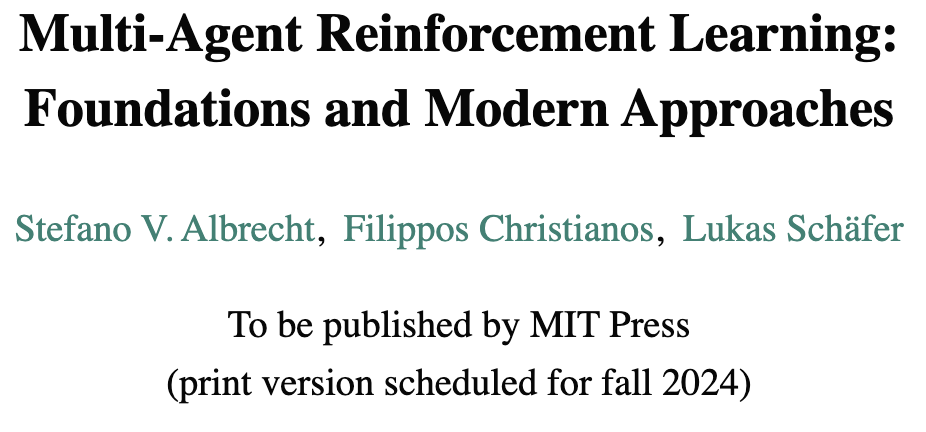
\includegraphics[width=\textwidth,height=.8\textheight,keepaspectratio]{images/1_MARL_book.png}
            
              \label{fig:enter-label}
            \end{figure}
          \end{column}
        
        \hspace{20pt}
            
          % Column for the text
            \begin{column}{0.45\textwidth}
	        \small

                This lecture is based on \textit{Multi-Agent Reinforcement Learning: Foundations and Modern Approaches} by Stefano V. Albrecht, Filippos Christianos and Lukas Sch\"afer
                
                \vspace{20pt}
                
                The book can be downloaded for free at \textcolor{blue}{\href{https://www.marl-book.com/}{www.marl-book.com}}.
            \end{column}
        
        \end{columns}
    \end{frame}
}

\newcommand{\leoslide}{
  \author{Stefano V. Albrecht, Filippos Christianos, Lukas Sch\"afer \\ Slides by: Leonard Hinckeldey}
}

\newcommand{\otherslide}{
  \author{Stefano V. Albrecht, Filippos Christianos, Lukas Sch\"afer}
}
	
\title{Multi-Agent Reinforcement Learning}
\date{}

\hypersetup{
  pdfsubject = {Multi-Agent Reinforcement Learning},
}

\leoslide

\subtitle{Deep Reinforcement Learning}

\begin{document}
\maketitle

\introslide

\begin{frame}{\outline}

\blist
    \item Deep-Q learning
    \item Moving target problem
    \item Addressing correlations in consecutive experiences
    \item Policy gradient algorithms
    \item Concurrent training 
\elist
\end{frame}

\section{Deep Q-Learning}

\begin{frame}[t]{Deep Q-Learning}

For \fat{deep} Q-learning, we use a neural network to approximate the $Q$ function.
\vspace{5pt}
\begin{columns}
    \begin{column}{0.4\textwidth}
    \vspace{0pt}%
        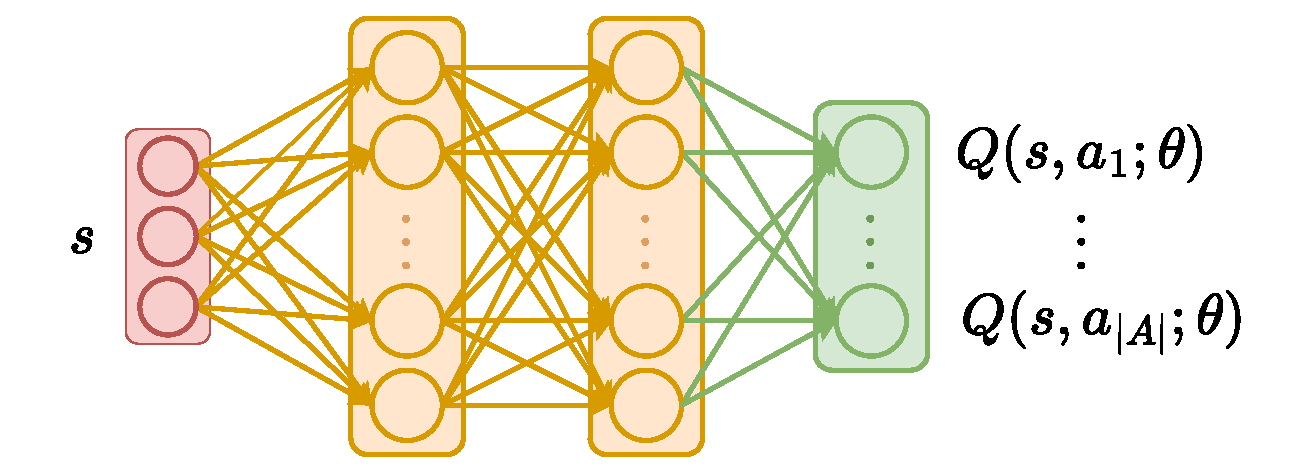
\includegraphics[width=\textwidth]{images/chapter_8/dqn_architecture.pdf}
    \end{column}\hfill
    \begin{column}{0.6\textwidth}
    \vspace{0pt}%
        \blist
            \item<1-> To train this we could define a loss function $\mathcal{L}(\theta) = \left(y^t - Q(s^t,a^t;\theta) \right)$
            \item<1-> But unlike supervised learning, we are not given $y^t$ beforehand
            \item <2->We can use the Q-learning update rule to define our $y^t$
        \elist
        \onslide<2->{\[
        y^t = 
        \begin{cases} 
        r^t & \text{if } s^{t+1} \text{ is terminal} \\
        r^t + \gamma \max_{a'} Q(s^{t+1}, a'; \theta) & \text{otherwise}
        \end{cases}
        \]}
    \end{column}    
\end{columns}   

  % \only<2>{
  %       \begin{tcolorbox}[colback=gray!5!white,colframe=yellow!75!black, title = Reminder]
  %       The Bellman update rule in tabular Q-learning is:
  %       \[
  %       Q(s^t, a^t) \leftarrow Q(s^t, a^t) + \alpha \left( r^t + \gamma \max_{a'} Q(s^{t+1}, a') - Q(s^t, a^t) \right)
  %       \]
  %       \end{tcolorbox}
  %       }

\end{frame}

% \begin{frame}{Naive Deep Q-Learning Pseudo-Code}
% \scalebox{0.75}{
% \begin{minipage}{0.7\linewidth}
% \balg{Deep Q-learning}{dql}
%     \State Initialise value network $Q$ with random parameters $\theta$
%     \State Repeat for every episode:
%     \For{time step $t=0, 1, 2, \dots$}
%         \State Observe current state $s^t$
%         \State With probability $\epsilon$: choose random action $a^t \in  A$
%         \State Otherwise: choose $a^t \in \argmax_{a}{Q(s^t, a; \theta)}$
%         \State Apply action $a^t$; observe reward $r^t$ and next state $s^{t+1}$
%         \If{$s^{t+1}$ is terminal}
%             \State Target $y^t \gets r^t$
%         \Else
%             \State Target $y^t \gets r^t + \dsc \max_{a'} Q(s^{t+1}, a'; \theta)$
%         \EndIf
%         % \State $y^t \gets \begin{cases}r^t & \text{if $s^{t+1}$ is terminal}\\ r^t + \dsc \max_{a'} Q(s^{t+1}, a'; \theta) & \text{otherwise}\end{cases}$
%         \State Loss $\mathcal{L}(\theta) \gets \left(y^t - Q(s^t, a^t; \theta)\right)^2$
%         \State Update parameters $\theta$ by minimising the loss $\mathcal{L}(\theta)$
%     \EndFor
% \ealg
% \end{minipage}%
%     }
% \end{frame}

\begin{frame}[t]{Naive Deep Q-Learning Pseudo-Code}
\vspace{-0.3cm}
\centering
\scalebox{0.8}{\begin{minipage}{0.95\linewidth}
\balg{Deep Q-learning}{dql}
    \State Initialize value network $Q$ with random parameters $\theta$
    \For{every episode}
        \For{time step $t=0, 1, 2, \dots$}
            \State Observe current state $s^t$
            \State With probability $\epsilon$: choose random action $a^t \in  A$
            \State Otherwise: choose $a^t \in \argmax_{a}{Q(s^t, a; \theta)}$
            \State Apply action $a^t$; observe reward $r^t$ and next state $s^{t+1}$
            \If{$s^{t+1}$ is terminal}
                \State Target $y^t \gets r^t$
            \Else
                \State Target $y^t \gets r^t + \gamma \max_{a'} Q(s^{t+1}, a'; \theta)$
            \EndIf
            % \State $y^t \gets \begin{cases}r^t & \text{if $s^{t+1}$ is terminal}\\ r^t + \dsc \max_{a'} Q(s^{t+1}, a'; \theta) & \text{otherwise}\end{cases}$
            \State Loss $\mathcal{L}(\theta) \gets \left(y^t - Q(s^t, a^t; \theta)\right)^2$
            \State Update parameters $\theta$ by minimising the loss $\mathcal{L}(\theta)$
        \EndFor
    \EndFor
\ealg
\end{minipage}%
    }

\vspace{.5em}

\visible<2->{
    This naive application of neural networks to RL algorithms has some problems.
}
    
\end{frame}

\begin{frame}[t]{The Moving Target Problem}

\vspace{-0.5em}

\begin{problembox}
    \e{Moving target problem} arises from the bootstrapped targets:
    \vspace{-1em}
    \[
        y^t = r^t + \gamma \max_{a'} Q(s^{t+1}, a'; \theta)
    \]
    \vspace{-2em}

    \visible<2->{
        \blist
            \item Value function with NNs generalize value estimates across inputs
            \item As targets $y^t$ depend on $\theta$, any update to $\theta$ changes the target
            \listtab This non-stationarity of the targets makes it difficult to learn optimal $\theta$
        \elist
    }
    \vspace{-0.4em}
\end{problembox}

\visible<3->{
    \begin{solutionbox}
        One solution is to use a \textbf{target network} with parameters $\bar{\theta}$ that are updated less often than our $Q$ network's parameters $\theta$  
    \end{solutionbox}
}
          
\end{frame}

\begin{frame}[t]{Correlation of Consecutive Experiences}

\blist
    \item Most ML algorithms using NNs assume i.i.d. data
    \item In RL, we collect data by interacting with an MDP with $s^{t+1} \sim \Stf(\st^t, \ac^t)$ $\rightarrow$ \fat{not} i.i.d
\elist
\vspace{0cm}
\only<1>{
    \begin{figure}[htbp]
        \centering
        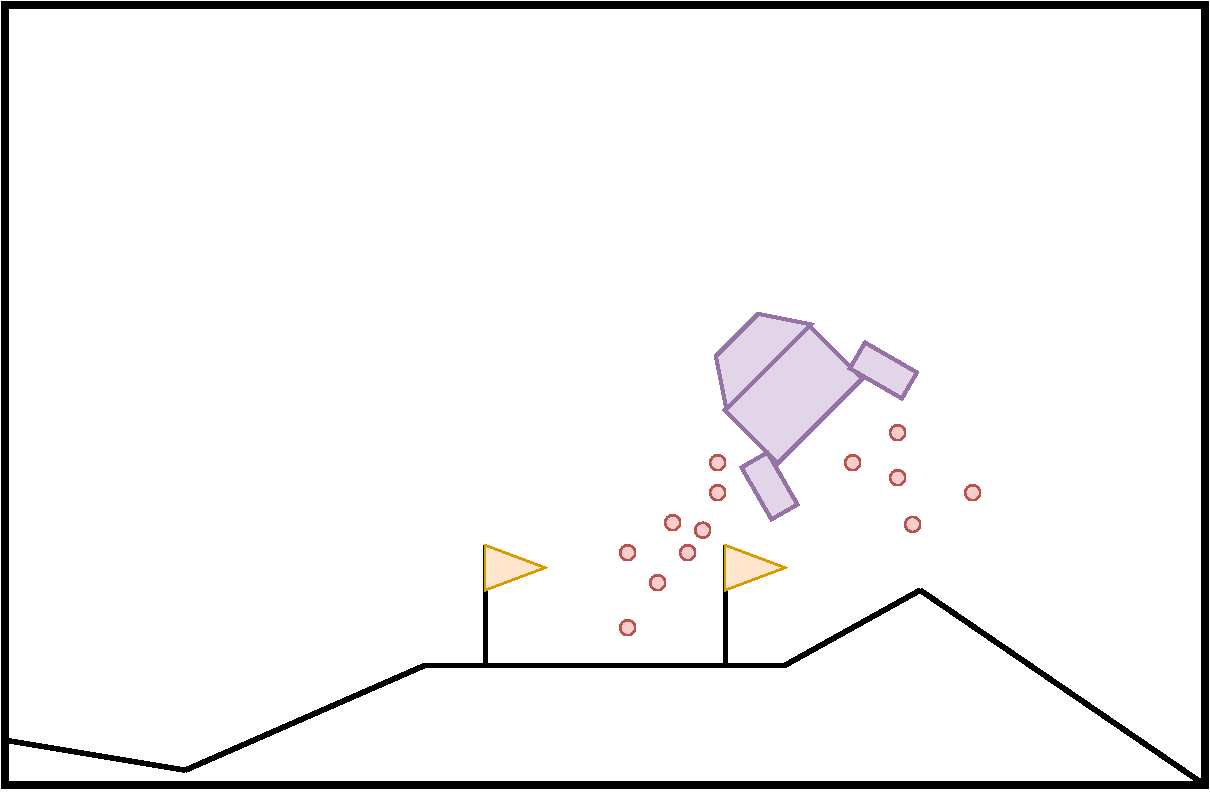
\includegraphics[width=0.25\textwidth, keepaspectratio]{images/chapter_8/lunarlander_right1.pdf}
        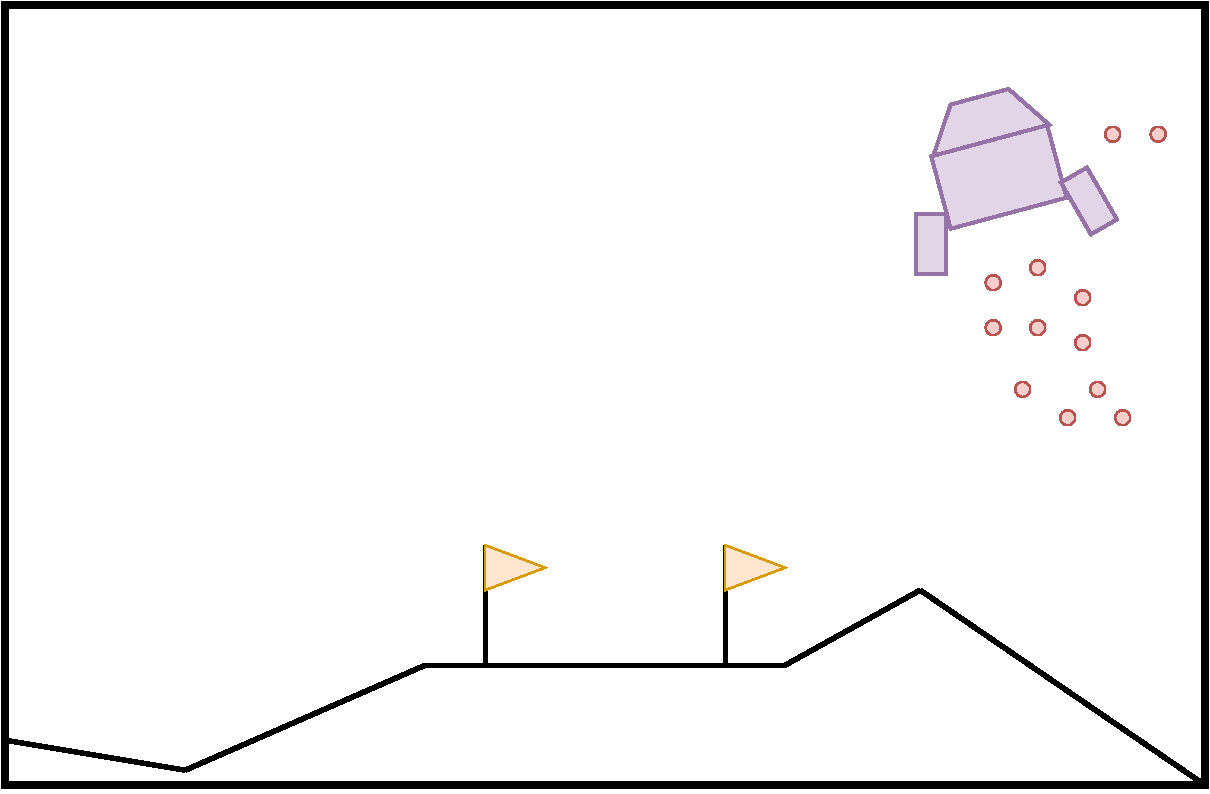
\includegraphics[width=0.25\textwidth, keepaspectratio]{images/chapter_8/lunarlander_right2.pdf}
        \begin{minipage}[c]{0.1\textwidth}
            \centering
            \Large $\cdots$
        \end{minipage}
        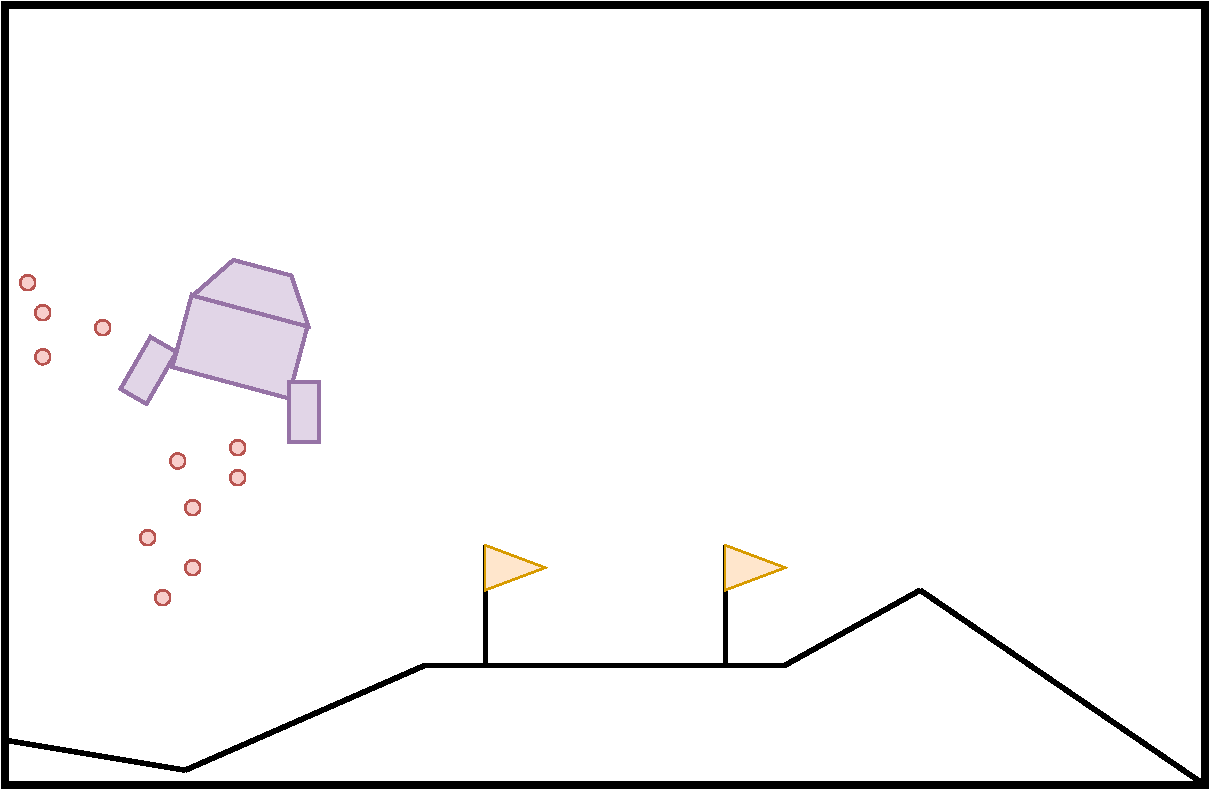
\includegraphics[width=0.25\textwidth, keepaspectratio]{images/chapter_8/lunarlander_left1.pdf}
    \end{figure}
}
\only<2->{
    \vspace{-.5em}

    \begin{figure}[htbp]
        \centering
        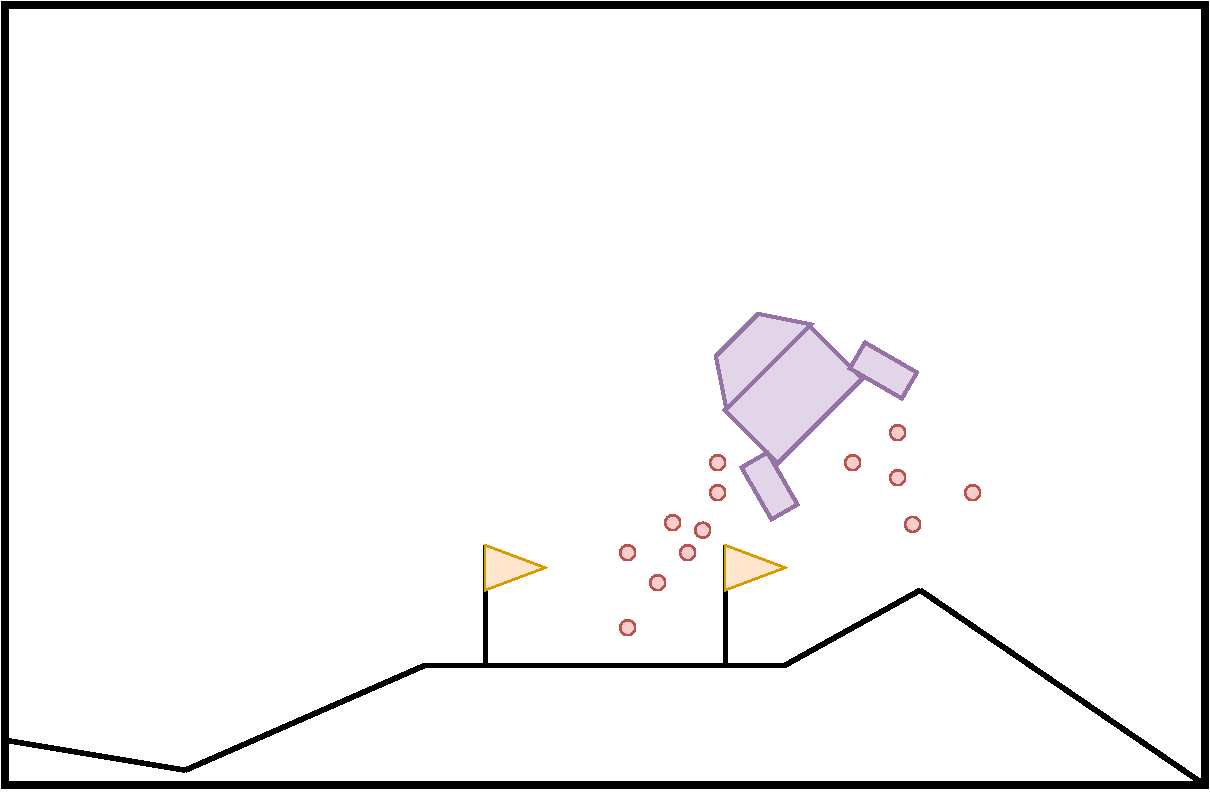
\includegraphics[width=0.15\textwidth]{images/chapter_8/lunarlander_right1.pdf}
        \begin{minipage}[c]{0.1\textwidth}
            \centering
            \Large $\cdots$
        \end{minipage}
        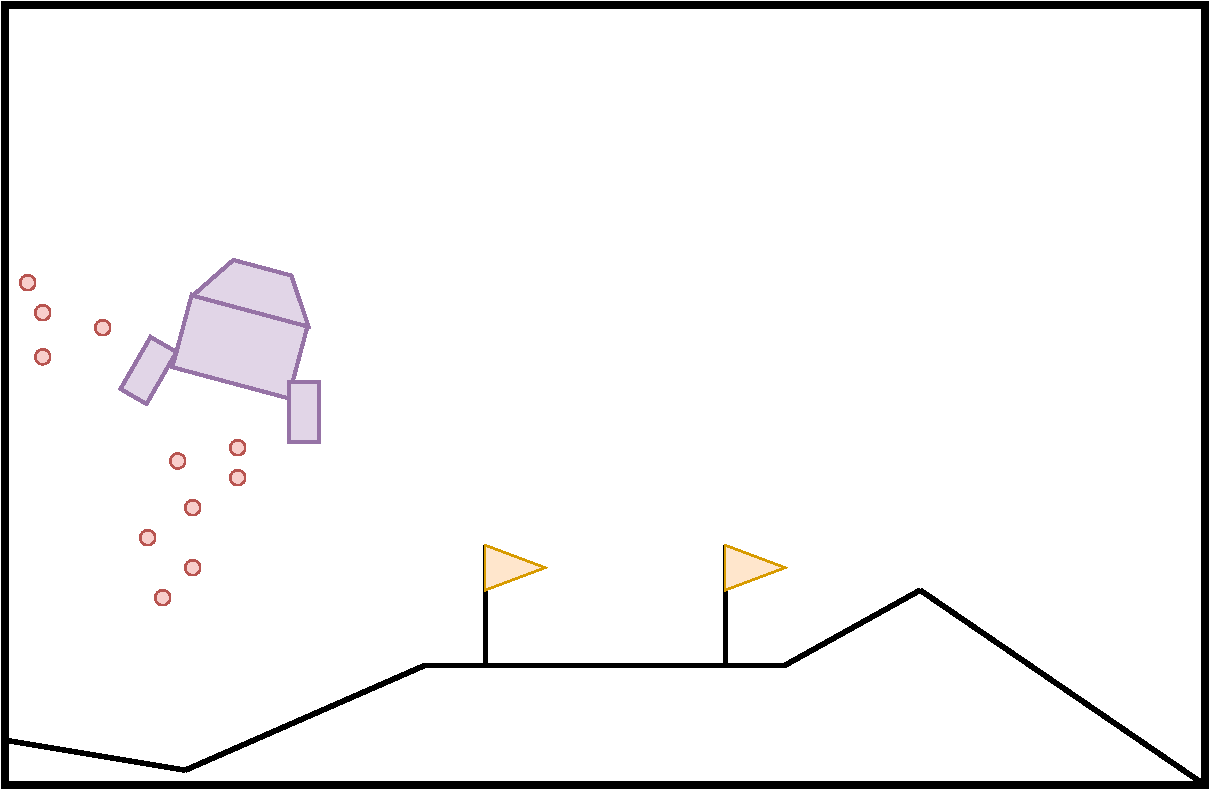
\includegraphics[width=0.15\textwidth]{images/chapter_8/lunarlander_left1.pdf}
    \end{figure}

    \vspace{-1.5em}
}

\visible<2->{
    \begin{problembox}
        This correlated data can lead to \fat{overfitting} of the value function to recent experiences, and result in \fat{catastophic forgetting} of previously learned estimates.
    \end{problembox}
}

\visible<3->{
    \begin{solutionbox}
        We train on samples of previous experiences stored in a \textbf{replay buffer}.
    \end{solutionbox}
}
    
\end{frame}


\begin{frame}[t]{Deep Q-Networks}

\textbf{Deep Q-networks} (DQN) is a foundational deep RL algorithm based on Q-learning.

\only<1>{
    \blist
        \item Tabular value function $\longrightarrow$ neural network
        \item Moving target problem $\longrightarrow$ target networks
        \item Correlated experiences $\longrightarrow$ replay buffer
    \elist
}

\only<2-5>{
    \fat{Target networks:}
    \blist
        \item<2-5> Compute target estimates with target network parameters $\bar{\theta}$:
            \vspace{-.5em}
            \[
                y^t \gets r^t + \gamma \max_{a'} Q(s^t+1, a'; \bar{\theta})
            \]
            \vspace{-2em}
        \item<3-5> Select actions according to the "main" value network $\rightarrow$ $a^t \in \arg\max_a Q(s^t, a; \theta)$
        \item<4-5> Update the "main" value network parameters $\theta$ by minimizing the DQL loss $\mathcal{L}(\theta)$
        \item<5> Update the \textbf{target network} parameters in regular intervals $\bar{\theta} \gets \theta$
    \elist
}
\only<6->{
    \fat{Replay buffers:}
    \only<6->{
        \blist
            \item<6-> Store experience tuples $(s^t, a^t, r^t, s^{t+1})$ in a replay buffer $\mathcal{D}$
            \item<7-> To compute the loss, sample batches of experience tuples (uniformly at random) from the replay buffer $\mathcal{B} \sim \mathcal{U}(\mathcal{D}$)
            \item<8-> Random sampling "breaks" correlations, allowing for a more stable optimization
            \item<9-> Also reuses experiences during training $\rightarrow$ improved sample efficiency
        \elist

        \vspace{-1em}

        \only<10>{
            \begin{notebox}
               Replay buffers can only be used for \textbf{off-policy} algorithms. We use experiences collected from previous (different) policies, which change as we update $\theta$.
            \end{notebox}
        }
    }
}

\end{frame}

\begin{frame}{DQN Pseudo Code}
    \vspace{-0.2cm}
    \centering
    \scalebox{0.7}{\begin{minipage}{\linewidth}
    \balg{Deep Q-networks (DQN)}{dqn}
        \State Initialize value network $Q$ with random parameters $\theta$
        \State Initialize target network with parameters $\bar{\theta} = \theta$
        \State Initialize an empty replay buffer $\mathcal{D} = \{\}$
        \For{every episode}
            \For{time step $t=0, 1, 2, \dots$}
                \State Observe current state $s^t$
                \State With probability $\epsilon$: choose random action $a^t \in  A$
                \State Otherwise: choose $a^t \in \argmax_{a}{Q(s^t, a; \theta)}$
                \State Apply action $a^t$; observe reward $r^t$ and next state $s^{t+1}$
                \State Store transition $(s^t, a^t, r^t, s^{t+1})$ in replay buffer $\mathcal{D}$
                \State Sample random mini-batch of $B$ transitions $(s^{k}, a^{k}, r^{k}, s^{k+1})$ from $\mathcal{D}$
                \If{$s^{k+1}$ is terminal}
                    \State Targets $y^k \gets r^k$
                \Else
                    \State Targets $y^k \gets r^k + \gamma \max_{a'} Q(s^{k+1}, a'; \bar{\theta})$
                \EndIf
                % \State $y_k \gets \begin{cases}\rew_k & \text{if $s'_k$ is terminal}\\ \rew_k + \dsc \max_{a'} Q(s'_k, a'; \widebar{\theta}) & \text{otherwise}\end{cases}$
                \State Loss $\mathcal{L}(\theta) \gets \frac{1}{B} \sum_{k=1}^B \left(y^k - Q(s^k, a^k; \theta)\right)^2$
                \State Update parameters $\theta$ by minimising the loss $\mathcal{L}(\theta)$
                \State In a set interval, update target network parameters $\bar{\theta}$
            \EndFor
        \EndFor
    \ealg
    \end{minipage}%
    }
\end{frame}

\begin{frame}[t]{Overestimation Bias}

\begin{problembox}
    DQN tends to \textbf{overestimate} values with 1-step targets
    \vspace{0pt}
    \[
    y^k \gets r^k + \gamma \max_{a'} Q(s^{k+1}, a'; \bar{\theta})
    \]

    \only\blist
        \item Using the $\max$ operator, select the maximum value estimate for the target 
        \item Since our value estimates do not necessarily reflect the true value function, the $\max$ operation will likely select an overestimated action-value estimate
        \item  This can slow down the convergence of the algorithm as the agent spends too much time exploring states with overestimated values
    \elist
\end{problembox}

\end{frame}

\begin{frame}[t]{Double Q-Learning}

\begin{solutionbox}
    \fat{Double Q-learning} reduces this overestimation bias by decoupling the action selection from value estimation using separate function approximations.

    \blist
        \item This can be achieved with minimal changes in DQN
        \item DDQN  uses the primary Q-network (with parameters $\theta$) to select actions while using the target network (with parameters $\bar{\theta}$) to estimate action values
        \item The target thus becomes:
    \elist
    \vspace{0pt}
    \[
    y^t = \begin{cases} 
    r^t & \text{if } s^{t+1} \text{ is terminal} \\
    r^t + \gamma Q(s^{t+1}, \arg\max_{a'} Q(s^{t+1}, a'; \theta); \bar{\theta}) & \text{otherwise}
    \end{cases}
    \]
\end{solutionbox}
    
\end{frame}

\begin{frame}{Deep Q-learning in Practice}

\begin{figure}[htbp]
\centering

\subfloat[Single-agent level-based foraging environment]{
    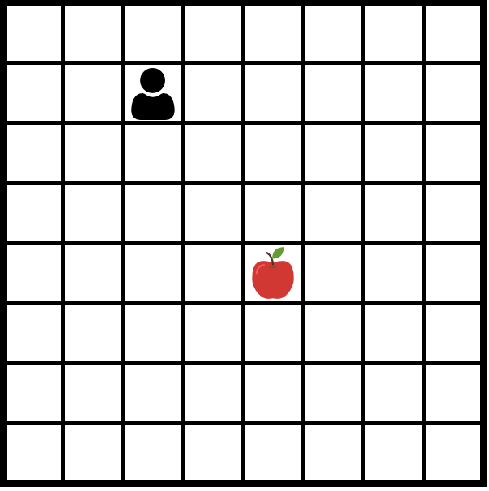
\includegraphics[width=0.3\textwidth]{images/chapter_8/single_agent_lbf_nolevel.pdf} % Replace with the path to your image
    % \label{fig:foraging_env}
}
\hspace{3em} % This adds some horizontal space between the subfigures
\visible<2->{
    \subfloat[Learning curves]{
        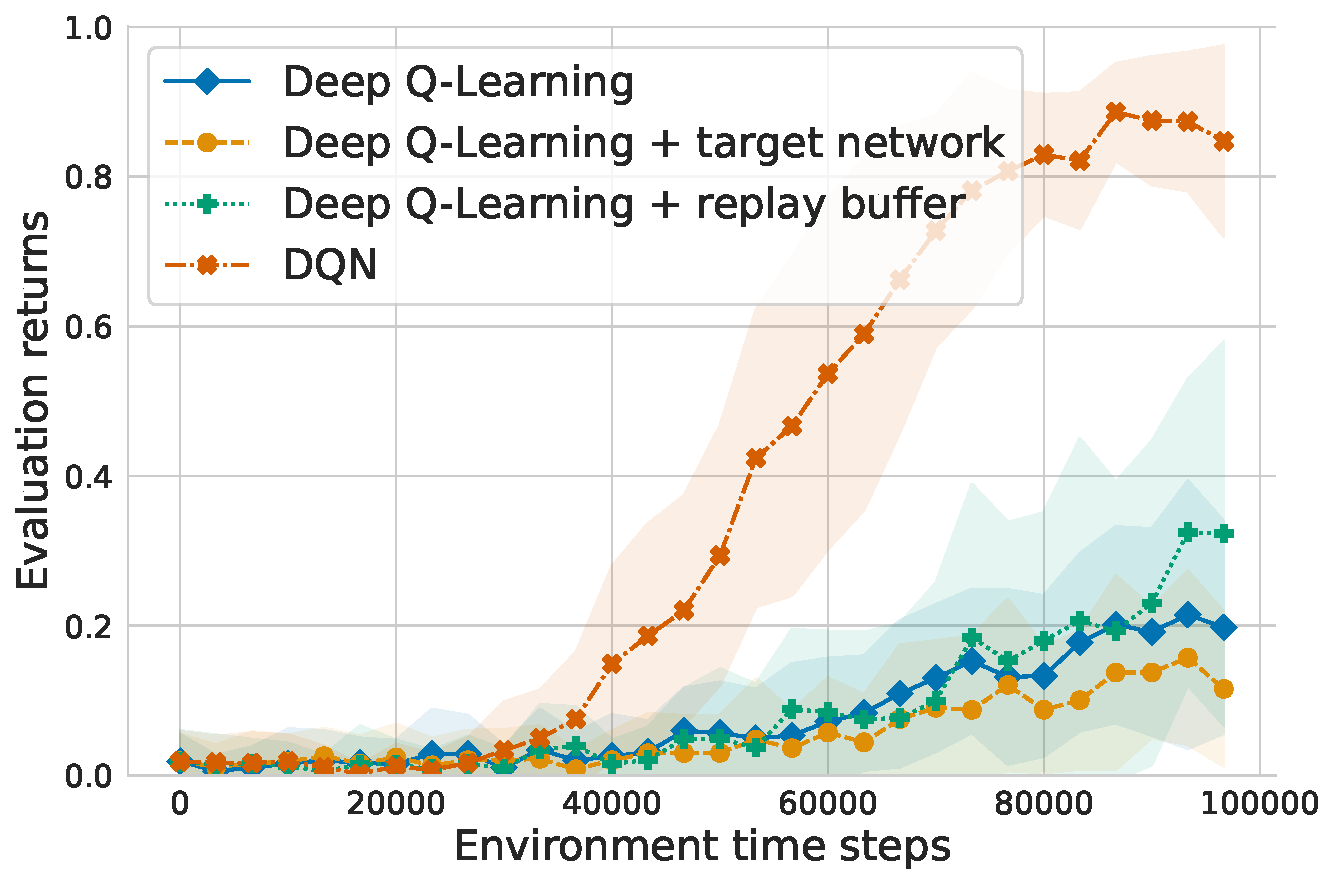
\includegraphics[width=0.5\textwidth]{images/chapter_8/vb_lbf_returns.pdf} 
        % \label{fig:learning_curves}
    }
}

\end{figure}
\vspace{2pt}

\visible<3->{
    Note that in isolation, neither the addition of \fat{target networks} nor of a \fat{replay buffer} are sufficient to stably train the agent with deep Q-learning in this environment.
}


% \begin{columns}[T] % The [T] alignment option aligns the columns' content at the top

% \begin{column}{.48\textwidth}
%     \centering
%     \includegraphics[width=\linewidth]{path_to_your_image_a} % Replace with the path to your image
%     \captionof{figure}{Single-agent level-based foraging environment}
%     \label{fig:foraging_env}
% \end{column}
% \hfill % Optional: could use \hspace{.04\textwidth} to add custom spacing
% \begin{column}{.48\textwidth}
%     \centering
%     \includegraphics[width=\linewidth]{path_to_your_image_b} % Replace with the path to your image
%     \captionof{figure}{Learning curves}
%     \label{fig:learning_curves}
% \end{column}

% \end{columns}

\end{frame}

\section{Policy Gradient Algorithms}

\begin{frame}[t]{Policy Gradients}

We considered a parameterized value function, but we can also directly parameterize the policy $\pi$.

\blist
    \item Use a NN for policy $\pi$ with parameters $\phi$
    \item Policy network receives state $s$ as input and outputs a scalar value for each action
    \item Scalars $l(s, a)$ represent the preference of the policy to select action $a$ in state $s$
    \item<2-> Preferences are then transformed into a probability distribution across the action space using a \fat{softmax} function:
\elist

\vspace{-1em}

\visible<2->{
    \[
        \pi(a \mid s; \phi) = \frac{e^{l(s,a;\phi)}}{\sum_{a' \in A} e^{l(s,a';\phi)}}
    \]
}
    
\end{frame}

\begin{frame}{Advantages of Learning a Policy}
    
% Using policy gradient algorithms has some notable advantages:

% \blist
%     \item It allows us to represent any probabilistic policy 
%     \item It's effective at representing policies for continuous action spaces
% \elist
\vspace{0.5cm}
\onslide<1->{\begin{minipage}{.5\textwidth}
\centering
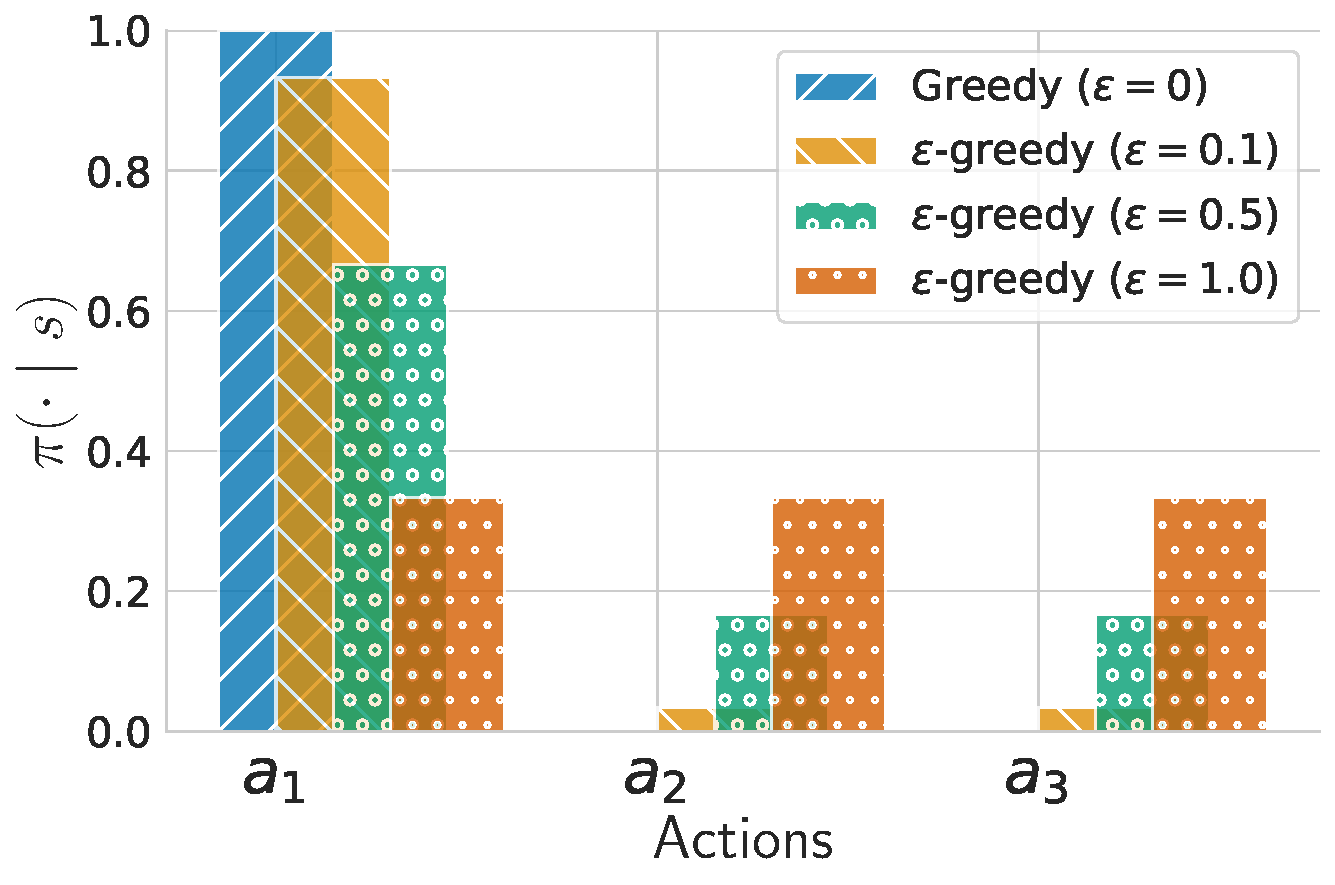
\includegraphics[width=.8\linewidth]{images/chapter_8/epsilon_greedy_policies.pdf} % Adjust size as needed
\\\textbf{$\epsilon$-greedy policies}  % Optional caption
\end{minipage}}%}
\onslide<2->{\begin{minipage}{.5\textwidth}
\centering
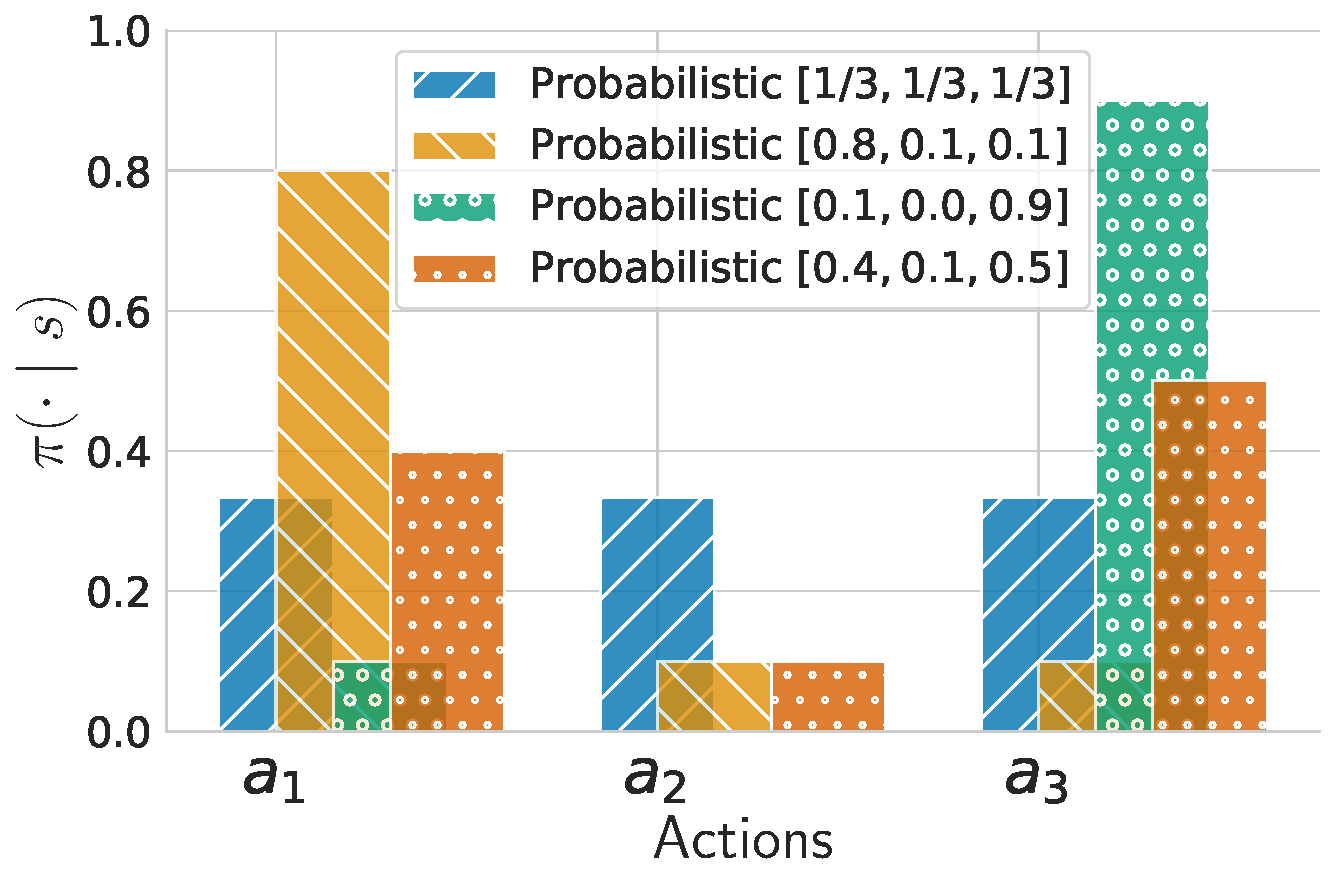
\includegraphics[width=.8\linewidth]{images/chapter_8/softmax_policy.pdf} % Adjust size as needed
\\\textbf{Probabilistic policies} % Optional caption
\end{minipage}}
\vspace{0.3cm}
\blist
    \item<1-> $\epsilon$-greedy policies struggle to represent diverse probabilistic policies
    \item<2-> Policy gradient algorithms allow us to represent \textbf{any} probabilistic policy
    \item<3-> Policy gradients are also effective for representing {\bf continuous} action spaces
\elist

\end{frame}

\begin{frame}[t]{Policy Gradient Theorem}

How to update parameters $\phi$ of the policy? Using the \textbf{policy gradient theorem}, we can express the gradient of the performance of a policy with respect to the parameter $\phi$ of the policy.
\[
\nabla_{\phi} J(\phi) \propto \sum_{s \in S} \Pr(s \mid \pi) \sum_{a \in A} Q^{\pi}(s, a) \nabla_{\phi} \pi(a \mid s; \phi)
\]

\only<1>{
\blist
    \item $J$ is a function measuring the quality of policy $\pi$
    \item $Pr(s \mid \pi)$ is the state-visitation distribution for policy $\pi$
    \item $Q^\pi(s, a)$ is the value for a given action and state under $\pi$
    \item The $J$ function is similar to a loss function, with the difference that we aim to \textbf{maximize} rather than minimize it
\elist
}

\only<2->{
\begin{notebox}
    The policy gradient theorem assumes that $Pr(s \mid \pi)$ are given under the currently optimized policy $\pi$ $\rightarrow$ this needs \fat{on-policy} data
\end{notebox}
}

\end{frame}

\begin{frame}[t]{Policy Gradient Theorem -- Continued}

The assumption that $Pr(s\mid \pi)$ is \textbf{on-policy} becomes apparent through a simple derivation.
\vspace{0pt}
\begin{align*}
\nabla_{\phi} J(\phi) &\propto \sum_{s \in S} \Pr(s \mid \pi) \sum_{a \in A} Q^{\pi}(s, a) \nabla_{\phi} \pi(a \mid s; \phi) \\
\visible<2->{&= \mathbb{E}_{a \sim \pi(\cdot \mid s; \phi)} \left[ \sum_{a \in A} Q^{\pi}(s, a) \nabla_{\phi} \pi(a \mid s; \phi) \right]} \\
\visible<3->{&= \mathbb{E}_{a \sim \pi(\cdot \mid s; \phi)} \left[ \sum_{a \in A} \pi(a \mid s; \phi) Q^{\pi}(s, a) \frac{\nabla_{\phi} \pi(a \mid s; \phi)}{\pi(a \mid s; \phi)} \right] \\
\visible<4->{&= \mathbb{E}_{a \sim \pi(\cdot \mid s; \phi)} \left[Q^{\pi}(s, a) \frac{\nabla_{\phi} \pi(a \mid s; \phi)}{\pi(a \mid s; \phi)} \right]}} \\
\visible<5->{&= \mathbb{E}_{a \sim \pi(\cdot \mid s; \phi)} \left[ Q^{\pi}(s, a) \nabla_{\phi} \log \pi(a \mid s; \phi) \right]} \\
\end{align*}
\end{frame}

% \begin{align*}
% \nabla_{\phi} J(\phi) &\propto \sum_{s \in S} \Pr(s \mid \pi) \sum_{a \in A} Q^{\pi}(s, a) \nabla_{\phi} \pi(a \mid s; \phi) \\
% &= \only<2->{\mathbb{E}_{a \sim \pi(\cdot \mid s; \phi)} \left[ \sum_{a \in A} Q^{\pi}(s, a) \nabla_{\phi} \pi(a \mid s; \phi) \right]} \\
% &= \only<3->{\mathbb{E}_{a \sim \pi(\cdot \mid s; \phi)} \left[ \sum_{a \in A} \pi(a \mid s; \phi) Q^{\pi}(s, a) \frac{\nabla_{\phi} \pi(a \mid s; \phi)}{\pi(a \mid s; \phi)} \right] \\
% &= \only<4->{\mathbb{E}_{a \sim \pi(\cdot \mid s; \phi)} \left[Q^{\pi}(s, a) \frac{\nabla_{\phi} \pi(a \mid s; \phi)}{\pi(a \mid s; \phi)} \right]}} \\
% &= \only<5->{\mathbb{E}_{a \sim \pi(\cdot \mid s; \phi)} \left[ Q^{\pi}(s, a) \nabla_{\phi} \log \pi(a \mid s; \phi) \right]} \\
% \end{align*}

\begin{frame}{Policy Gradient Theorem -- Continued}

\begin{intuitionbox}
    \[
        \nabla_{\phi} J(\phi) \propto \mathbb{E}_{a \sim \pi(\cdot \mid s; \phi)} \left[Q^{\pi}(s, a) \frac{\nabla_{\phi} \pi(a \mid s; \phi)}{\pi(a \mid s; \phi)} \right]
    \]
    \vspace{.3em}

    We can interpret the components of the policy gradient theorem as follows:
    \blist
        \item<1->  $\nabla_{\phi} \pi(a \mid s; \phi)$: gradient of $\phi$ pointing in the direction that most increase the probability of taking action $a$ when in state $s$
        \item<2->  $Q^{\pi}(s, a)$: expected returns as a quality measure of taking action $a$ in state $s$
        \item<3-> $\frac{1}{\pi(a \mid s; \phi)}$: normalization coefficient to account for varying probabilities of different actions under the policy
    \elist
\end{intuitionbox}

    
\end{frame}

\begin{frame}[t]{REINFORCE: Monte Carlo}

To apply the policy gradient theorem, we must find a way to derive expected returns.

\blist
    \item \textbf{REINFORCE} is a policy gradient algorithm that uses Monte Carlo (MC) to estimate the expected returns of a policy
    \item<2-> The algorithm minimizes the following loss for an episodic history $h = \{s^0, a^0, r^0, ... ,s^{T-1}, a^{T-1}, r^{T-1}, s^T\}$:
\elist
\vspace{0pt}
\visible<2->{
    \[
        \mathcal{L}(\phi) = - \frac{1}{T}\sum_{t=0}^{T-1}\left(\sum_{\tau = 1}^{t-1}\gamma^{\tau-1}\mathcal{R}(s^\tau, a^\tau, s^{\tau+1})\right) \log \pi(a^t \mid s^t; \phi)
    \]
}

\blist
    \item<3-> Note this loss has a negative sign, as we want to \textbf{maximize} expected returns
\elist    
\end{frame}

\begin{frame}[t]{REINFORCE Pseudocode}

\balg{REINFORCE}{reinforce}
    \State Initialize policy network $\pi$ with random parameters $\phi$
    \For{every episode}
        \For{time step $t=0, 1, 2, \dots, T - 1$}
            \State Observe current state $s^t$
            \State Sample action $a^t \sim \pi(\cdot \mid s^t; \phi)$
            \State Apply action $a^t$; observe reward $r^t$ and next state $s^{t+1}$
        \EndFor
        % \State Collect history $\fhis \gets \{s^0, \ob^0, a^0, \ldots, s^{T-1}, \ob^{T-1}, a^{T-1}, s^T, \ob^T\}$
        % \State Collect history $\{s^0, a^0, \ldots, s^{T-1}, a^{T-1}, s^T\}$
        % \State $\phi \gets \phi - \alpha \nabla_\phi \loss\left(\phi \mid \batch = \his \right)$ (loss from \Cref{eq:reinforce-loss})

        % \State Loss $\loss(\phi) \gets - \frac{1}{T} \sum_{t=0}^{T-1} \left(\sum_{\tau=t}^{T-1} \dsc^{\tau-t} \Rew(s^{\tau}, a^{\tau}, s^{\tau+1})\right) \log \pi(a^t \mid s^t; \phi)$
        \State Loss $\mathcal{L}(\phi) \gets - \frac{1}{T} \sum_{t=0}^{T-1} \left(\sum_{\tau=t}^{T-1} \gamma^{\tau-t} r^\tau\right) \log \pi(a^t \mid s^t; \phi)$
        \State Update parameters $\phi$ by minimizing the loss $\mathcal{L}(\phi)$
    \EndFor
\ealg

\end{frame}

\begin{frame}[t]{Baseline to Reduce Variance}

\begin{problembox}
    High variance of MC estimates causes unstable gradients and training.
\end{problembox}

\visible<2->{
    \begin{solutionbox}
        \blist
            % \item MC estimates are high-variance as they depend on all the states and  actions encountered during an episode
            \item One way to reduce variance is subtract a \textbf{baseline} from the return estimates
            \item A common choice of baseline is a state-value function $V(s)$ which can be trained to minimize the loss $\mathcal{L}(\theta) = \frac{1}{T}\sum_{t=1}^{T-1}(u(h^t)-V(s^t; \theta))^2$
            \item The REINFORCE policy loss would then become 
        \elist
        \[
        \mathcal{L}(\phi) = - \frac{1}{T}\sum_{t=0}^{T-1}\left(u(h^t)-V(s^t; \theta)\right)log \pi(a^t \mid s^t; \phi)
        \]
    \end{solutionbox}
}
    
\end{frame}

\begin{frame}[t]{Baselines Continued}
The inclusion of the baseline does not affect the gradients in expectation:
\vspace{-0em}
\begin{align*}
    \nabla_\phi J(\phi)  &\propto \sum_{s\in S} \text{Pr}(s \mid \pi) \sum_{a\in A} \left(Q^\pi(s, a) - b(s)\right) \nabla_\phi \pi(a \mid s; \phi)\\
    % &= \mathbb{E}_{\pi}\left[{\sum_{a\ina} \left(Q^\pi(s, a) - b(s)\right) \nabla_\phi \pi(a \mid s; \phi)}\right]\\
    % &= \mathbb{E}_{\pi}{\sum_{a\ina} \pi(a \mid s; \phi) \left(Q^\pi(s, a) - b(s)\right) \frac{\nabla_\phi \pi(a \mid s; \phi)}{\pi(a \mid s; \phi)}}\\
    % &= \mathbb{E}_{\pi}{\left(Q^\pi(s, a) - b(s)\right) \frac{\nabla_\phi \pi(a \mid s; \phi)}{\pi(a \mid s; \phi)}}\\
    \visible<2->{&= \mathbb{E}_{\pi}\left[{\left(Q^\pi(s, a) - b(s)\right) \nabla_\phi \log \pi(a \mid s; \phi)}\right]}\\
    % &= \mathbb{E}_{\pi}{Q^\pi(s, a) \nabla_\phi \log \pi(a \mid s; \phi) - b(s) \nabla_\phi \log \pi(a \mid s; \phi)}\\
    \visible<3->{&= \mathbb{E}_{\pi}\left[{Q^\pi(s, a) \nabla_\phi \log \pi(a \mid s; \phi)}\right] - \mathbb{E}_{\pi}\left[{b(s) \nabla_\phi \log \pi(a \mid s; \phi)}\right]}\\
    % &= \mathbb{E}_{\pi}\left[{Q^\pi(s, a) \nabla_\phi \log \pi(a \mid s; \phi)} - \sum_{s \in S} \text{Pr}(s \mid \pi) \sum_{a\ina} b(s) \nabla_\phi \pi(a \mid s; \phi)\right]\\
    % &= \mathbb{E}_{\pi}{Q^\pi(s, a) \nabla_\phi \log \pi(a \mid s; \phi)} - \sum_{s \in S} \text{Pr}(s \mid \pi) b(s) \sum_{a\ina} \nabla_\phi \pi(a \mid s; \phi)\\
    \visible<4->{&= \mathbb{E}_{\pi}\left[{Q^\pi(s, a) \nabla_\phi \log \pi(a \mid s; \phi)}\right] - \sum_{s \in S} \text{Pr}(s \mid \pi) b(s) \nabla_\phi \sum_{a\in A} \pi(a \mid s; \phi)}\\
    \visible<5->{&= \mathbb{E}_{\pi}\left[{Q^\pi(s, a) \nabla_\phi \log \pi(a \mid s; \phi)}\right] - \sum_{s \in S} \text{Pr}(s \mid \pi) b(s) \nabla_\phi 1}\\
    \visible<6->{&= \mathbb{E}_{\pi}\left[{Q^\pi(s, a) \nabla_\phi \log \pi(a \mid s; \phi)}\right]- \sum_{s \in S} \text{Pr}(s \mid \pi) b(s) 0}\\
    \visible<7->{&= \mathbb{E}_{\pi}\left[{Q^\pi(s, a) \nabla_\phi \log \pi(a \mid s; \phi)}\right]}
    \label{eq:policy-gradient-baseline}
\end{align*}
    
\end{frame}

\begin{frame}{Actor-Critic Algorithms}

The policy gradient theorem allows us to optimize our parameterized policy; we still need to approximate expected returns. 

\blist
    \item MC methods have high variance and require an entire episode to compute estimates
    \item \textbf{Actor-critic} algorithms aim to reduce variance and update more often by using  \textbf{bootstrapped return estimates}
\elist
\vspace{-.5cm}
\begin{align*}
\mathbb{E}_{\pi} \left[ u(h^{t}) \mid s^{t} \right] &= \mathbb{E}_{\pi} \left[ R(s^{t}, a^{t}, s^{t+1}) + \gamma u(h^{t+1}) \mid s^{t}, a^{t} \sim \pi( \cdot \mid s^{t}) \right] \\
&= \mathbb{E}_{\pi} \left[ R(s^{t}, a^{t}, s^{t+1}) + \gamma V(s^{t+1}) \mid s^{t}, a^{t} \sim \pi( \cdot  \mid s^{t}) \right]    
\end{align*}

\blist
    \item We now train a \textbf{critic} (value function approximator) alongside the \textbf{actor} (parameterized policy) which acts as a baseline
\elist

\end{frame}

\begin{frame}[t]{Balancing Bias and Variance}
\vspace{-1em}

\begin{problembox}
    MC estimates have high \fat{variance} and bootstrapping introduces \fat{bias} since the value function might not yet approximate the true expected returns.
\end{problembox}

\visible<2->{
    \begin{solutionbox}
        \fat{N-step returns} allow us to balance between bias and variance:
        \vspace{0pt}
        \[
            \ex{\pi}{u(\his^t) \mid \st^t} = \ex{\pi}{\left( \sum_{\tau=0}^{N-1} \gamma^{\tau} \mathcal{R}(s^{t+\tau}, a^{t+\tau}, s^{t+\tau+1}) \right) + \gamma^N V(s^{t+N}) \Bigg| s^t, a^{\tau} \sim \pi(\cdot \mid s^{\tau})}
        \]

        $N = 1 \rightarrow$ one-step bootstrapped returns \ $\ldots$ \ $N = T \rightarrow$ MC returns
    \end{solutionbox}
}
\end{frame}

\begin{frame}[t]{Balancing Bias and Variance -- Continued}
    \begin{figure}
        \centering
        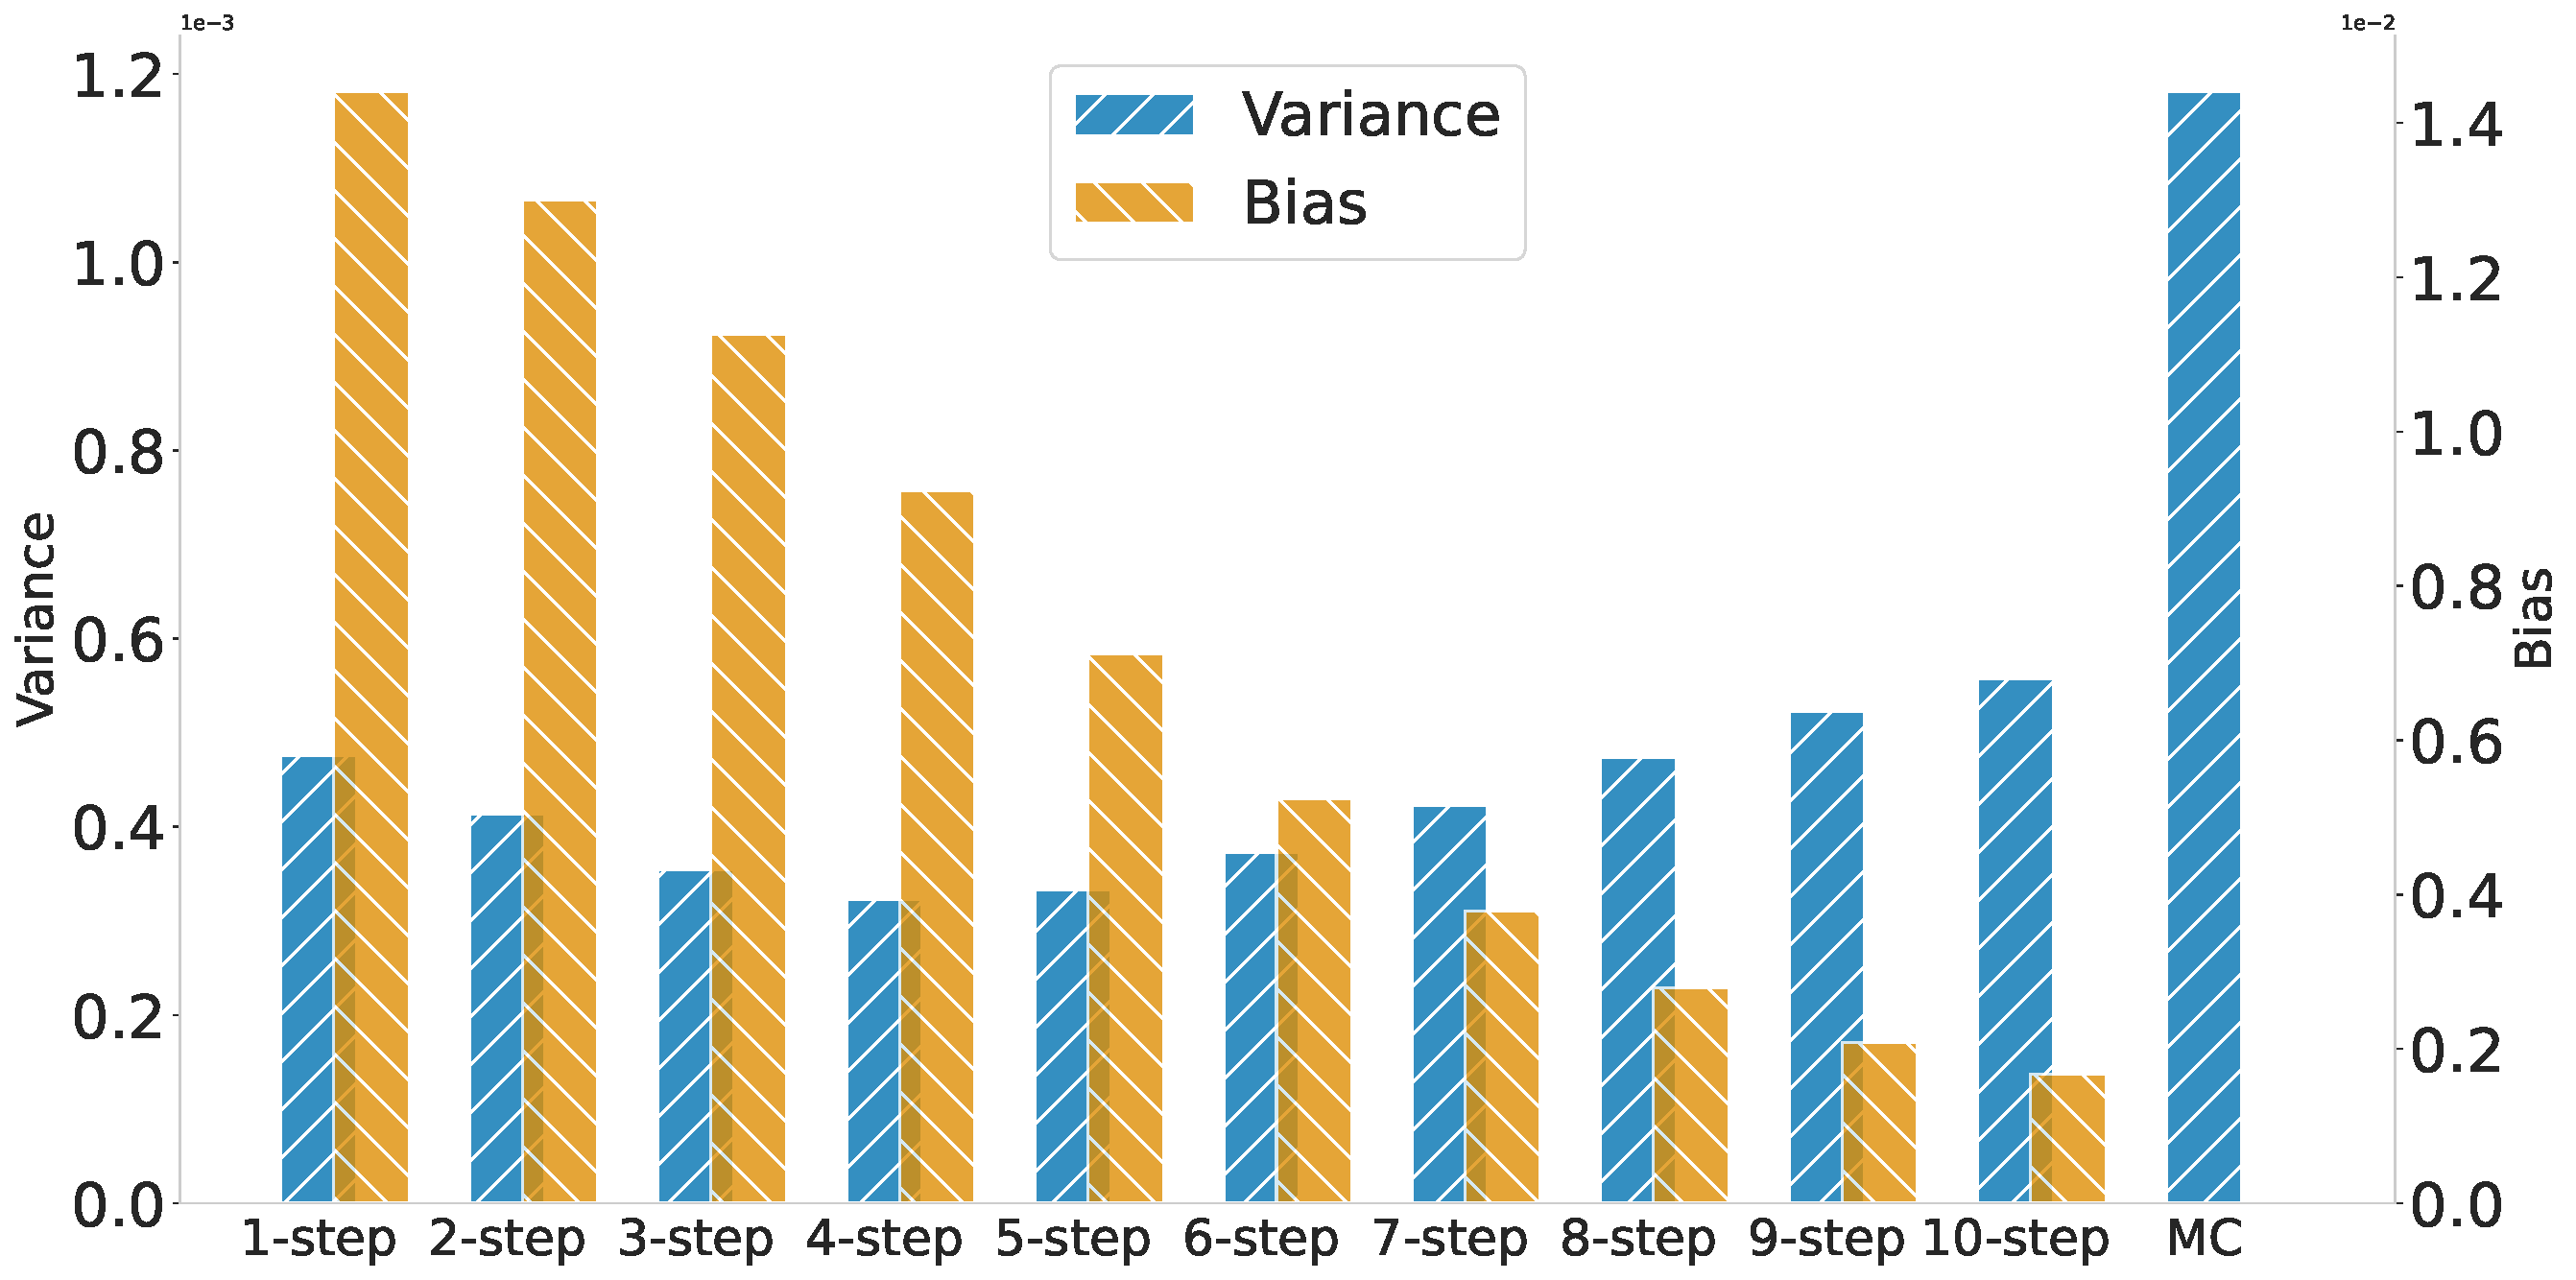
\includegraphics[width=0.9\textwidth]{images/chapter_8/a2c_lbf_nstep_comparison.pdf}
    \end{figure}
\end{frame}

\begin{frame}[t]{Advantage Actor Critic (A2C)}

Advantage actor-critic is a foundation actor-critic algorithm which uses the \textbf{advantage} of a policy to guide the policy gradients.

\blist
    \item The advantage is defined as
\elist
\vspace{0pt}
\[
    Adv^{\pi}(s, a) = Q^{\pi}(s, a) - V^{\pi}(s) = \rew + 
\]

\visible<2->{
    \blist
        \item We can compute the advantage using only a state-value function:
    \elist
    \vspace{0pt}
    \[
    Adv(s^t, a^t) = Q(s^t, a^t) - V(s^t) = 
    \begin{cases} 
    r^t - V(s^t) & \text{if } s^{t+1} \text{ is terminal} \\
    r^t + \gamma V(s^{t+1}) - V(s^t) & \text{otherwise} 
    \end{cases}
    \]
    \blist
        \item<3-> We can also still use N-step returns to reduce bias during the advantage computation
    \elist
}
\end{frame}

\begin{frame}{A2C Pseudocode}
\vspace{-0.2cm}
\centering
\scalebox{0.725}{\begin{minipage}{\linewidth}
\balg{A2C}{a2c}
\State Initialize actor network $\pi$ with random parameters $\phi$
\State Initialize critic network $V$ with random parameters $\theta$
\For{every episode}
    \For{time step $t=0, 1, 2, \dots$}
        \State Observe current state $s^t$
        \State Sample action $a^t \sim \pi(\cdot \mid s^t; \phi)$
        \State Apply action $a^t$; observe reward $r^t$ and next state $s^{t+1}$
        \If{$s^{t+1}$ is terminal}
            \State Advantage $Adv(s^t, a^t) \leftarrow r^t - V(s^t; \theta)$
            \State Critic target $y^t \leftarrow r^t$
        \Else
            \State Advantage $Adv(s^t, a^t) \leftarrow r^t + \gamma V(s^{t+1}; \theta) - V(s^t; \theta)$
            \State Critic target $y^t \leftarrow r^t + \gamma V(s^{t+1}; \theta)$
        \EndIf
        \State Actor loss $\mathcal{L}(\phi) \leftarrow -Adv(s^t, a^t) \log \pi(a^t \mid s^t; \phi)$
        \State Critic loss $\mathcal{L}(\theta) \leftarrow (y^t - V(s^t; \theta))^2$
        \State Update parameters $\phi$ by minimizing the actor loss $\mathcal{L}(\phi)$
        \State Update parameters $\theta$ by minimizing the critic loss $\mathcal{L}(\theta)$
    \EndFor
\EndFor
\ealg
\end{minipage}}
\end{frame}

\begin{frame}[t]{Proximal Policy Optimization (PPO)}
    \vspace{-1em}

    \begin{problembox}
        Policy gradient methods can cause significant shifts in the policy with a single update which can worsen the policy!
    \end{problembox}

    \begin{solutionbox}
        Limit the change of the policy in a single update $\rightarrow$ \textbf{trust region} of a policy
    \end{solutionbox}

    \e{Proximal policy optimization} (PPO) computes an efficient surrogate objective to limit the change in the policy when executing multiple updates:
    \begin{equation*}
        \mathcal{L}(\phi) = - \min\left(
            \begin{array}{ll}
                \rho(\st^t, \ac^t) Adv(\st^t, \ac^t),\\
                \text{clip}\left(\rho(\st^t, \ac^t),1 - \epsilon, 1 + \epsilon\right) Adv(\st^t, \ac^t)
            \end{array}
        \right)
    \end{equation*}
\end{frame}

\begin{frame}[t]{PPO Surrogate Objective}
\begin{equation*}
    \mathcal{L}(\phi) = - \min\left(
        \begin{array}{ll}
            \rho(\st^t, \ac^t) Adv(\st^t, \ac^t),\\
            \text{clip}\left(\rho(\st^t, \ac^t),1 - \epsilon, 1 + \epsilon\right) Adv(\st^t, \ac^t)
        \end{array}
    \right)
\end{equation*}

\blist
    \item $\rho$ represents the importance sampling ratio $\rho(s, a) = \frac{\pi(a \mid s; \phi)}{\pi_\beta(a \mid s)}$
    \item $\pi_\beta$ represents the behavior policy followed to select action $\ac^t$ in state $\st^t$
    \item $\epsilon$ is a hyperparameter that determines the allowed change of the policy
\elist

\visible<2->{
    Importance sampling ratios serves multiple purposes:

    \blist
        \item Correct for differences in data distributions of $\pi_\beta$ and $\pi$
        \item Represent measure of divergence between $\pi_\beta$ and $\pi$ $\rightarrow$ can be clipped to limit divergence
    \elist
}

    
\end{frame}

\begin{frame}[t]{PPO Pseudocode}
\vspace{-1em}
\scalebox{0.6}{\begin{minipage}{.8 \linewidth}
\balg{Simplified proximal policy optimization (PPO)}{ppo}
    \State Initialize actor network $\pol$ with random parameters $\phi$
    \State Initialize critic network $V$ with random parameters $\theta$
    \For{every episode}
        \For{time step $t=0, 1, 2, \dots$}
            \State Observe current state $\st^t$
            \State Sample action $\ac^t \sim \pol(\cdot \mid \st^t; \phi)$
            \State Apply action $\ac^t$; observe reward $\rew^t$ and next state $\st^{t+1}$
            % \State $\pol_\beta \gets \pol(\cdot; \phi)$
            \State $\pol_\beta(\ac^t \mid \st^t) \gets \pol(\ac^t \mid \st^t; \phi)$
            \For{epoch $e=1, \dots, N_e$}
                \State $\rho(\st^t, \ac^t) \gets \pol(\ac^t \mid \st^t; \phi) \div \pol_\beta(\ac^t \mid \st^t)$

                \If{$\st^{t+1}$ is terminal}
                    \State Advantage $Adv(\st^t, \ac^t) \gets \rew^t - V(\st^t; \theta)$
                    \State Critic target $y^t \gets r^t$
                \Else
                    \State Advantage $Adv(\st^t, \ac^t) \gets \rew^t + \dsc V(\st^{t+1}; \theta) - V(\st^t; \theta)$
                    \State Critic target $y^t \gets \rew^t + \dsc V(\st^{t+1}; \theta)$
                \EndIf
                % \State $Adv(\st^t, \ac^t) \gets \begin{cases}\rew^t - V(\st^t) & \text{if $\st^{t+1}$ is terminal}\\ \rew^t + \dsc V(\st^{t+1}) - V(\st^t) & \text{otherwise}\end{cases}$
                % \State $y^t \gets \begin{cases}\rew^t & \text{if $\st^{t+1}$ is terminal}\\ \rew^t + \dsc V(\st^{t+1}; \theta) & \text{otherwise}\end{cases}$
                \State Actor loss $\loss(\phi) \gets - \min\left(
                    \begin{array}{ll}
                        \rho(\st^t, \ac^t) Adv(\st^t, \ac^t),\\
                        \text{clip}\left(\rho(\st^t, \ac^t),1 - \epsilon, 1 + \epsilon\right) Adv(\st^t, \ac^t)
                    \end{array}
                \right)$
                \State Critic loss $\loss(\theta) \gets \left(y^t - V(\st^t; \theta)\right)^2$
                \State Update parameters $\phi$ by minimising the actor loss $\loss(\phi)$
                \State Update parameters $\theta$ by minimising the critic loss $\loss(\theta)$
            \EndFor
        \EndFor
    \EndFor
\ealg
\end{minipage}}
\hfill
\begin{minipage}{.4\textwidth}
    \blist
        \item PPO executes multiple epochs of updates!
        \item For first epoch, $\pi = \pi_\beta$ \listtab $\rho = 1$
        \item After first epoch, $\pi \neq \pi_\beta$ \listtab needs $\rho$ to correct for off-policy data
    \elist
\end{minipage}
    
\end{frame}

\begin{frame}{Policy Gradient Algorithms in Practice}
\setcounter{subfigure}{0}
\begin{figure}[htbp]
\centering

\subfloat[Single-agent level-based foraging environment]{
    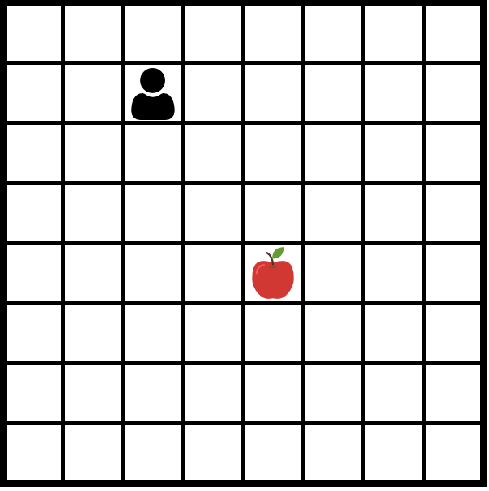
\includegraphics[width=0.3\textwidth]{images/chapter_8/single_agent_lbf_nolevel.pdf} % Replace with the path to your image
    % \label{fig:foraging_env}
}
\hfill % This adds some horizontal space between the subfigures
\subfloat[Learning curves]{
    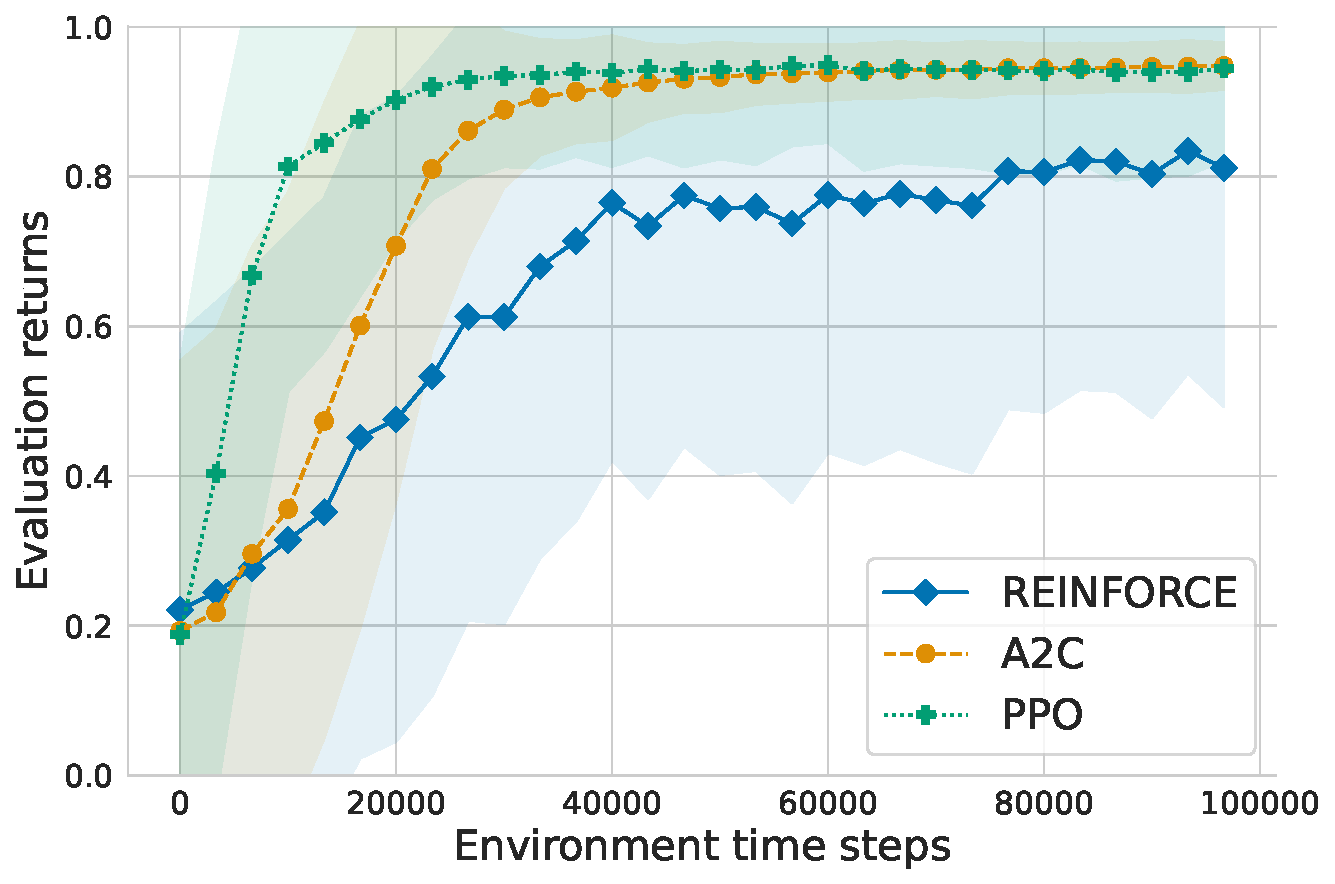
\includegraphics[width=0.6\textwidth]{images/chapter_8/pg_lbf_returns.pdf} 
    % \label{fig:learning_curves}
}

\end{figure}
\vspace{2pt}
    
\end{frame}

\section{Concurrent Training}

\begin{frame}{Concurrent Training of Policies}

Policy gradient algorithms rely on on-policy data, which raises the question of how to deal with correlation in the collected data and how to increase sample efficiency. 

\blist
    \item Concurrent training of policies speeds up training by getting more samples (in parallel), leading to better gradients and breaking of correlation of data
    \item There are many ways to achieve this, but there are two simple methods commonly used, \textbf{synchronous training} and \textbf{asynchronous training}
\elist
    
\end{frame}

\begin{frame}{Synchronous Training}

\begin{columns}
    \begin{column}{0.5\textwidth}
    \begin{figure}
        \centering
        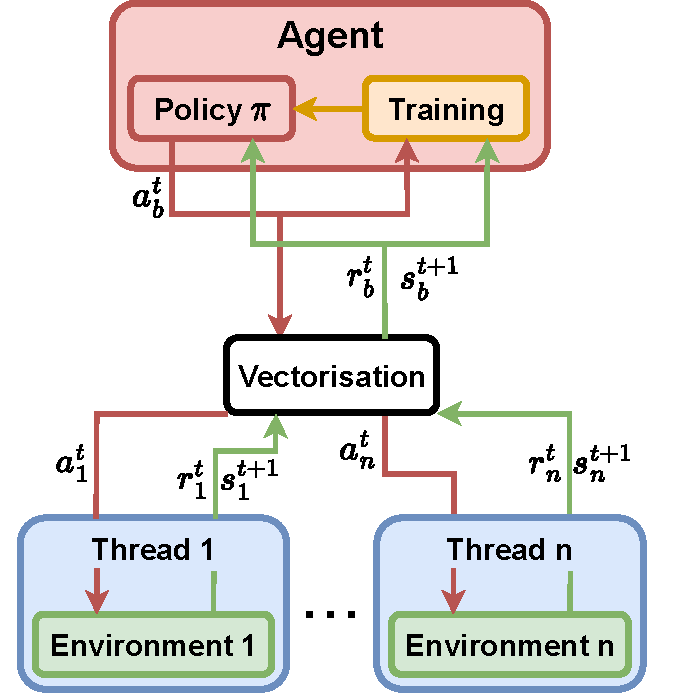
\includegraphics[width=0.9\textwidth]{images/chapter_8/synchronous_training.pdf}
        \label{fig:enter-label}
    \end{figure}
    \end{column}
    \begin{column}{0.5\textwidth}
        \blist
            \item Initiates separate instances of the environment in separate threads
            \item At each timestep, the agent receives a batch of states and rewards from each thread
            \item The agent then independently chooses an action for each thread/environment
            \item Aggregate gradients across batch of experiences $\rightarrow$ more stable and efficient optimization
        \elist
    \end{column}
\end{columns}
\end{frame}

\begin{frame}{Asynchronous Training}
\vspace{2pt}
\begin{columns}
    \begin{column}{0.5\textwidth}
    \begin{figure}
        \centering
        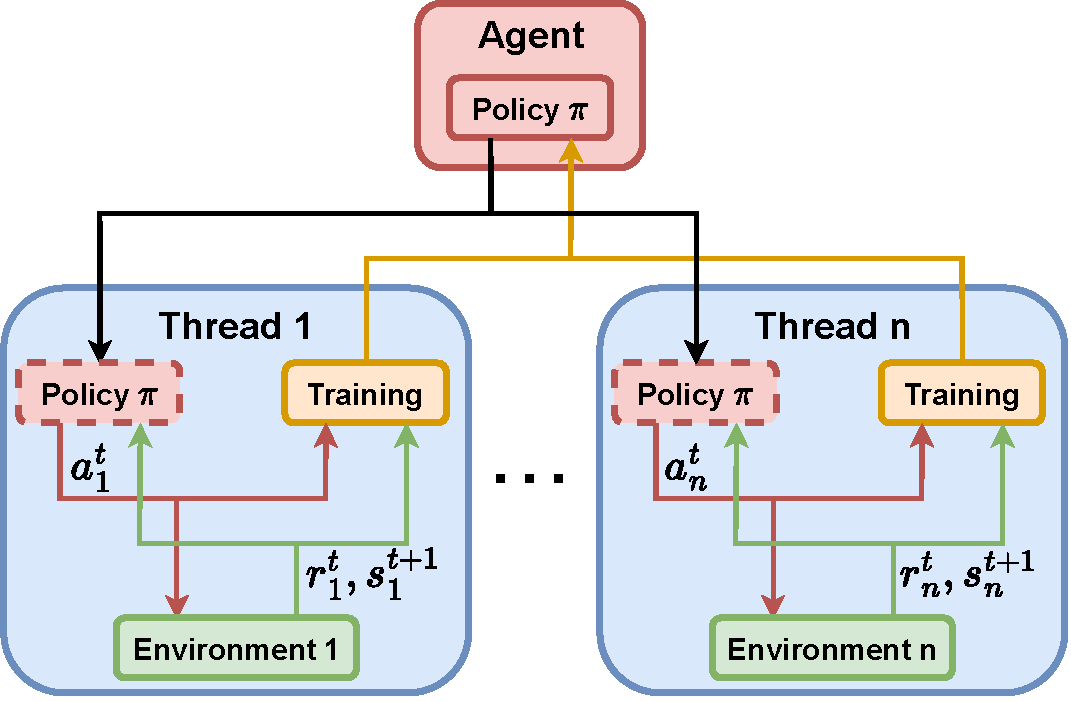
\includegraphics[width=0.9\textwidth]{images/chapter_8/asynchronous_training.pdf}
        \label{fig:enter-label}
    \end{figure}
    \end{column}
    \begin{column}{0.5\textwidth}
        \blist
            \item Asynchronous training parallelizes the optimization of the agent.
            \item Each thread separately computes the loss and gradients and optimizes the parameters of the agent's network 
            \item Once gradients are computed, the central agent's network is updated
            \item Asynchronous training is particularly effective if multiple accelerators (e.g. GPUs) are available
        \elist
    \end{column}
\end{columns}
\end{frame}

\begin{frame}{Observation, States, and Histories in Practice}

We have thus far only considered algorithms that condition on the entire states of the environment, in practice we however often have \textbf{partial observability}.

\begin{columns}
    \begin{column}{0.4\textwidth}
        \begin{figure}
            \centering
            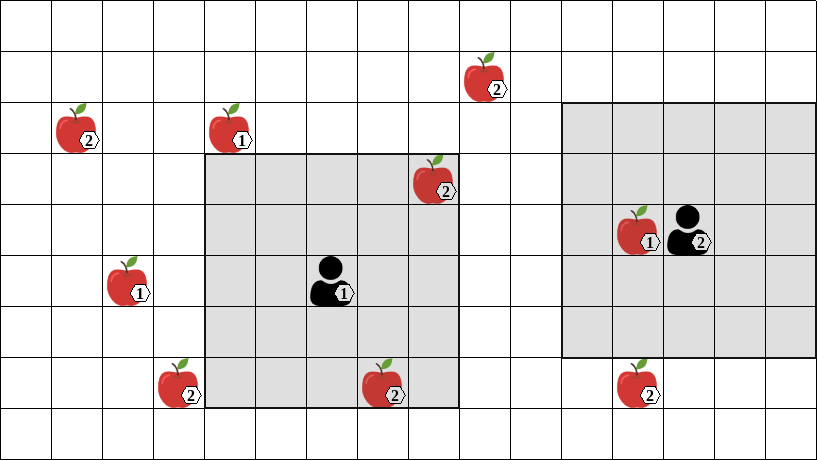
\includegraphics[width=0.9\textwidth]{images/environments/lbf/foraging_po.png}
        \end{figure}
        We want to condition value functions and policies on observation history $h^t = (o^0, ..., o^t)$
    \end{column}
    \begin{column}{0.6\textwidth}
        \blist
            \item<2-> Feedforward NN assume constant input size, this would require zero-padding vectors to the maximum episode length
            \item<2-> Zero-padding requires knowledge about maximum episode length and results in high-dimensional and sparse inputs
            \item<3-> To avoid this we can use RNNs that process sequences of observations with one observation at a time while maintaining the previous history in the hidden state
        \elist
    \end{column}
\end{columns}

\end{frame}

% \begin{frame}{Observation, States, and Histories in Practice}
%
% We have thus far only considered algorithms that condition on the entire states of the environment, in practice we however often have \textbf{partial observability}.
%
% \begin{columns}
% \begin{column}{0.6\textwidth}
%     \blist
%     \item Condition on the history of observations $h^t = (o^0, ..., o^t)$
%     \item Feedforward NNs assume constant input size $\longrightarrow$ requires zero-padding vectors to maximum episode length
%     \item Zero-padding $\longrightarrow$ high-dimensional sparse inputs
%     \item Can use RNNs, feeding in 1 observation at a time while updating the hidden state to represent information about the entire history
%     \elist
% \end{column}
% \end{columns}
% \end{frame}

\begin{frame}{Summary}

\fat{We covered:}
    \blist
        \item Deep Q-learning
        \item Moving-target problem and correlations of consecutive experiences
        \item Policy gradient algorithms
        \item Concurrent training of policies
        \item Observation, states, and histories under partial observability
    \elist

\fat{Next we'll cover:}

    \blist
        \item Multi-agent deep reinforcement learning 
    \elist
    
\end{frame}

\end{document}
